\chapter{PLOS CB Paper}

\section{Introduction}

DNA, the material basis of genetic information, is a flexible polymer comprising two strands of nucleotides that coil around each other, at a rate of 10.5 base pairs per turn.
When subjected to torsional stress, DNA can either writhe around itself, forming 3-dimensional loops, or twist more or less tightly than in its relaxed state~\citep{krogh2018}; both forms are referred to as DNA supercoiling ($\sigma$).
DNA is said to be positively supercoiled ($\sigma > 0$) when it is overwound around itself, and negatively supercoiled ($\sigma < 0$) when it is underwound; bacterial DNA is normally maintained in a moderately negatively supercoiled state, with a reference value of $\sigma=-0.066$ in \emph{Escherichia coli}~\citep{crozat2005}.
In bacteria, DNA supercoiling plays an important role in the regulation of gene expression~\citep{martisb.2019}, as DNA supercoiling is highly dynamic, in both space along the chromosome and time during the cell lifecycle~\citep{krogh2018}, and as the level of supercoiling at the promoter of a gene modulates the expression of that gene~\citep{forquet2021}.
Furthermore, gene transcription itself locally impacts the level of DNA supercoiling, resulting in an interplay between supercoiling and transcription~\citep{dorman2019}, hinting at a possible role for this coupling as an evolutionary force shaping genome organization~\citep{junier2016}.

\subsection{The Dynamic Nature of DNA Supercoiling}

At the local scale, DNA supercoiling is directly affected by gene transcription.
Indeed, when an RNA polymerase transcribes a gene, it experiences a rotational drag that hampers its rotation around the DNA molecule, and generates a buildup of positive supercoiling upstream, and negative supercoiling downstream, of the transcribed gene~\citep{liu1987,ma2016}.
This accumulation is partially resolved by topoisomerases, enzymes that alter DNA supercoiling by cutting and rotating the DNA strands~\citep*{duprey2021}.
The two main bacterial topoisomerases are gyrase, which dissipates positive supercoiling by introducing negative supercoils at an ATP-dependent rate, and topoisomerase I, which oppositely relaxes negative supercoiling~\citep{martisb.2019}.

At a larger scale, while supercoiling would propagate freely along the length of an unconstrained DNA molecule, many nucleoid-associated proteins (NAPs) such as FIS, H-NS or HU bind to bacterial DNA in addition to RNA polymerases, creating topological barriers to the propagation of supercoils~\citep{travers2005a}.
This can result in a DNA supercoiling gradient at the scale of the whole chromosome, from a negatively supercoiled origin of replication to a more relaxed end, such as in stationary phase \emph{E. coli}~\citep{lal2016}, exemplifying the dynamic character of DNA supercoiling in both time and space.

In bacteria, the level of DNA supercoiling can furthermore be affected by numerous environmental challenges.
Salt shock transiently increases negative DNA supercoiling in \emph{E. coli}~\citep{hsieh1991}; the acidic intracellular environment relaxes DNA in the facultative pathogen \emph{Salmonella enterica} var. Typhimurium~\citep{marshall2000}; and higher temperatures relax DNA in the plant pathogen \emph{Dickeya dadantii}~\citep{herault2014}, but increases negative supercoiling in the human pathogen \emph{Shigella flexneri}~\citep{tobe1995}.

\subsection{DNA Supercoiling and Gene Regulation}

Through its effect on gene transcription, the regulation of DNA supercoiling is a widespread mechanism for the control of bacterial gene expression.
In \emph{E. coli},~\cite{peter2004} showed that 7\% of genes were sensitive to a relaxation of chromosomal DNA, of which one third were up-regulated by relaxation and two thirds down-regulated.
Similar results were obtained for \emph{S. enterica}, in which 10\% of genes were sensitive to DNA relaxation~\citep{webber2013}, and for \emph{S. pneumoniae}, in which around 13\% of genes were sensitive to relaxation~\citep{ferrandiz2010}.
When instead inducing extreme negative supercoiling in \emph{D. dadantii}, 13\% of the genes in the exponential phase and 7\% in the stationary phase were affected~\citep{pineau2022}.
The regulatory role of DNA supercoiling might be especially important in bacteria with reduced genomes, such as the obligate aphid endosymbiotic bacterium \emph{Buchnera aphidicola}, which is nearly devoid of transcription factors~\citep{brinza2013}.

Moreover, selection can act on the level of DNA supercoiling in order to modulate the regulation of gene expression.
In the Long-Term Evolution Experiment (LTEE), 12 \emph{E. coli} populations were evolved for several tens of thousands of generations, in a glucose-poor environment~\citep{lenski1991}.
In 10 of these populations, an increase in fitness was indeed linked to mutations in the \emph{topA} and \emph{fis} genes, which regulate the level of DNA supercoiling~\citep{crozat2010}.
When inserted into the ancestral strain, these mutations increased the level of negative supercoiling as well as the bacterial growth rate~\citep{crozat2005}, demonstrating that the level of DNA supercoiling can indeed evolve as a response to new environments.

Finally, the regulation of gene expression by DNA supercoiling could be a force helping shape the evolution of bacterial genomes.
Indeed, supercoiling-sensitive genes tend to group in up or down-regulated clusters in \emph{E. coli}~\citep{peter2004}, \emph{S. enterica}~\citep{webber2013} and \emph{S. pneumoniae}~\citep{ferrandiz2010}, suggesting an adaptive role in the grouping together of these clusters.
Indeed, synteny segments, or clusters of neighboring genes that show correlated expression patterns, are evolutionarily conserved across the Gram-negative \emph{E. coli} and the distantly related Gram-positive \emph{Bacillus subtilis}~\citep{junier2016}, strengthening the hypothesis that these domains could play an important role in the regulation of bacterial gene expression.

\subsection{The Transcription-Supercoiling Coupling}

As we saw before, the process of transcribing a given gene generates an accumulation of positive supercoiling downstream of this gene, and of negative supercoiling upstream of this gene~\citep{liu1987}.
If another gene is located closely enough to this first gene, the change in supercoiling at the promoter of this gene will impact its transcription rate, as negative supercoiling increases promoter activity, and positive supercoiling decreases it~\citep{forquet2021}.
In turn, this second gene will also generate a change in supercoiling that affects the first gene, resulting in an interaction between the transcription levels of these two genes.
Depending on the relative orientation of these genes, several types of interactions are therefore possible: if the two genes lie in diverging orientations, they are both upstream of each other, and therefore reinforce each other's transcription in a positive feedback loop.
Conversely, if they lie in convergent orientations, on the contrary, each gene inhibits the transcription of the other gene.
Finally, if the genes lie in a tandem orientation, the downstream gene up-regulates the upstream gene, whereas the upstream gene down-regulates the downstream gene.

This effect, which has been called the transcription-supercoiling coupling~\citep{martisb.2019}, has been documented in several bacterial genetic systems.
In \emph{S. flexneri}, the \emph{virB} promoter is normally only active at high temperature, but can be activated at low temperature by the insertion of a phage promoter in divergent orientation~\citep{tobe1995}.
Similarly, the expression of the \emph{leu-500} promoter in \emph{S. enterica} can be increased or decreased by the insertion of upstream transcriptionally active promoters, depending on their relative orientation~\citep{elhanafi2000}.
The magnitude of this effect has been explored in a synthetic construct using the inducible \emph{ilvY} and \emph{ilvC} \emph{E. coli} promoters, inserted on a plasmid in divergent orientations.
In this system, a decrease in the activity of \emph{ilvY} is associated with a decrease in \emph{ilvC} activity, and an increase in \emph{ilvY} activity with an increase in \emph{ilvC} activity as well~\citep{rhee1999}.

There are, however, hints that the biological relevance of the transcription-supercoiling coupling might not be confined to a few specific cases.
Indeed, in \emph{E. coli}, the typical size of topological domains, inside which the supercoiling generated by gene transcription can propagate, is around 10kb~\citep{postow2004}.
As the average size of \emph{E. coli} genes is 1kb, and the average intergenic distance about 120bp~\citep{blattner1997}, this means that any single topological domain encompasses several genes that can potentially physically interact via the transcription-supercoiling coupling.
A statistical analysis of the relative position of neighboring on the \emph{E. coli} chromosome furthermore reveals shows that genes that are up-regulated by negative supercoiling have more neighbors in divergent orientations, while genes that are down-regulated by negative supercoiling have more neighbors in converging orientations~\citep{sobetzko2016}, suggesting that the transcription-supercoiling coupling plays a role in regulating the activity of these genes.

\paragraph{}

In this article, we present an individual-based evolutionary model of gene expression at the whole-genome scale, in which gene transcription is regulated only by DNA supercoiling, expanding upon earlier work~\citep{grohens2021}.
We expose individuals to different environmental conditions, represented by different levels of global supercoiling, and show that the same genome can display qualitatively different patterns of gene activation depending on the environment, and mediated by the transcription-supercoiling coupling between neighboring genes.
We then characterize the spatial organization of genes along the genome through which complex patterns of gene activation levels, mediated by the transcription-supercoiling coupling, can emerge, suggesting that this coupling could indeed have played an important role in the evolution of the topological domains that shape bacterial DNA.


\section{An Evolutionary Model of the Transcription-Supercoiling Coupling}
\label{sec:model}

The model we present in this section builds upon the proof-of-concept model presented in~\cite{grohens2021}.
The model is a two-level individual-based evolutionary simulation that aims at studying the evolutionary effect of the transcription-supercoiling coupling on genome structure.
The first level in the model describes the interaction between the transcription rates of genes on a genome mediated by supercoiling, and the other level describes the evolution of individual genomes under selection for specific gene transcription levels, with chromosomal inversions as the only source of mutation.

\subsection{Individual-Level Model}
\label{sec:indiv_model}

We define the genotype of an individual in our model as a single circular chromosome, representative of a bacterial chromosome.
The chromosome consists in a fixed number of protein-coding genes, which are separated by non-coding intergenic segments of varying sizes, and has a basal supercoiling level $\sigma_{basal}$.
Each gene on the chromosome is characterized by its starting position (genes cannot overlap in our model), its orientation (on the leading or lagging strand), its length, and its basal expression level.
The genome of an example individual with 20 genes is presented on the left-hand side of Figure~\ref{fig:random_indiv}.

We then define the phenotype of an individual as the stable state in the expression level of its genes, as they interact with each other through the transcription-supercoiling coupling.
The phenotype depends on the environment, which imposes a shift $\sigma_{env}$ to the DNA supercoiling level.
The right-hand side panel of Figure~\ref{fig:random_indiv} shows the computation of this stable state in a particular environment.
Note that, in this model and throughout this article, we conflate
gene transcription rates with mRNA concentrations, as we assume that mRNAs degrade at a constant rate, and as transcription rates in our model are only affected by the direct effect of supercoiling on transcription.
We furthermore conflate transcription rates with expression levels, as we again assume proteins to be translated at a rate proportional to the associated mRNA concentrations and degraded at a constant rate.

\begin{figure}[H]
  \centering
  \begin{subfigure}[t]{0.44\textwidth}
    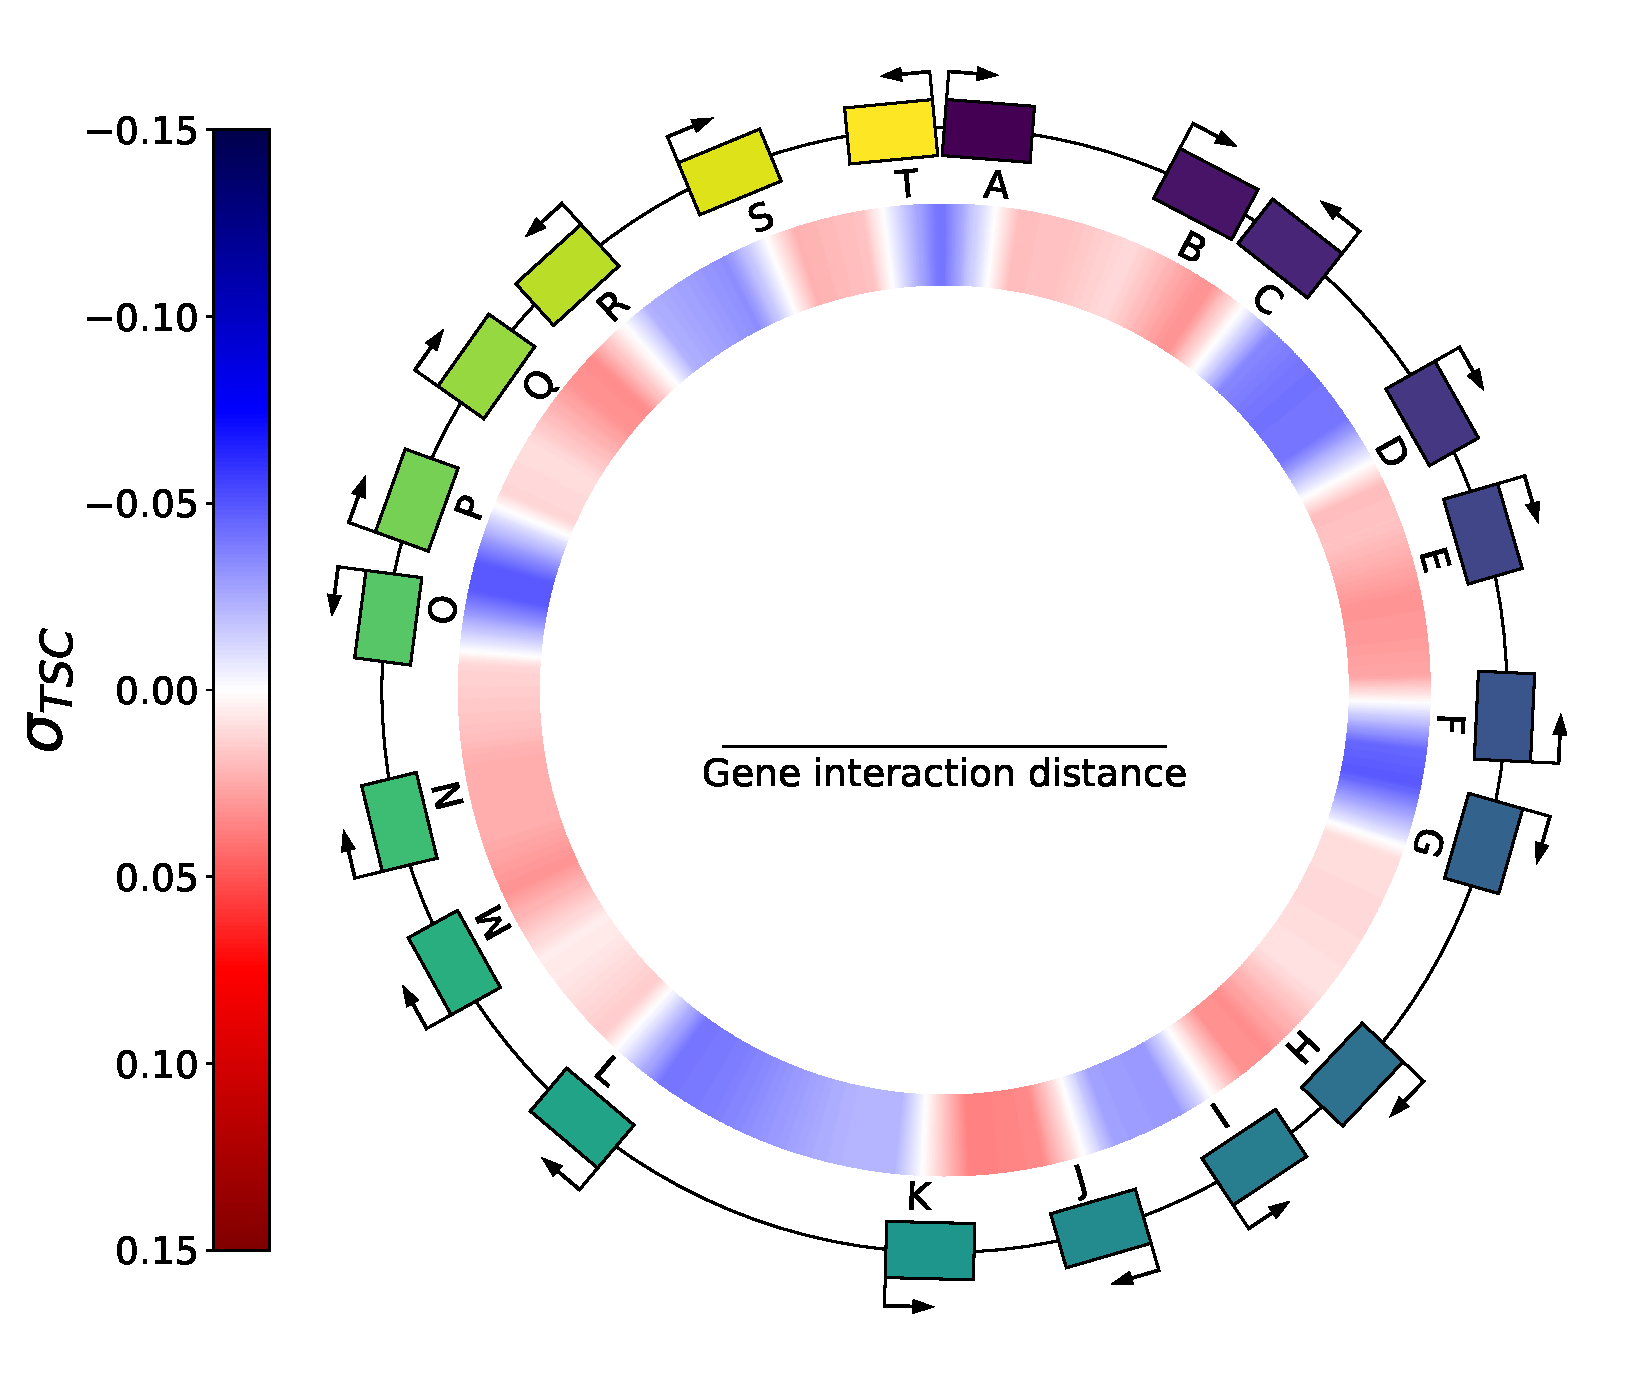
\includegraphics[width=\textwidth]{ploscb/img/random_genome_and_tsc.pdf}
    \label{subfig:random_genome}
  \end{subfigure}
  \begin{subfigure}[t]{0.55\textwidth}
    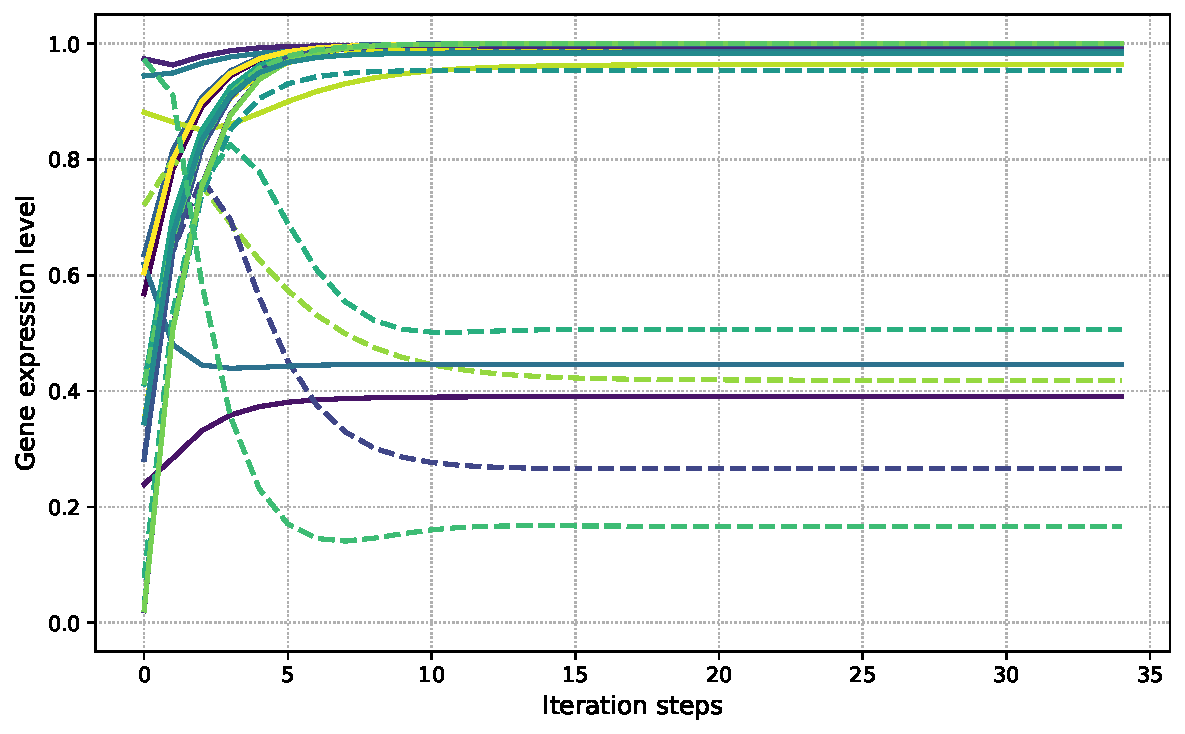
\includegraphics[width=\textwidth]{ploscb/img/random_gene_expr.pdf}
    \label{subfig:random_expr}
  \end{subfigure}
  \caption{Left: genome (outer ring) and stable-state level of transcription-generated supercoiling ($\sigma_{TSC}$, inner ring) of an example genome with 20 genes placed at random positions and orientations, with a gene length and average intergenic distance of 1 kb each, and a basal supercoiling level of $\sigma_{basal} = -0.066$.
  The individual is evaluated in an environment in which $\sigma_{env} = 0$.
  We can observe a buildup in negative supercoiling (blue) between divergently oriented genes, and a buildup in positive supercoiling (red) between convergently oriented genes.
  Right: evolution of the expression level of each gene of the individual during the computation of their stable state, starting from random initial values.
  Dashed lines represent genes on the lagging strand.}
  \label{fig:random_indiv}
\end{figure}

\paragraph{Effect of Transcription on Supercoiling}
For an individual with a genome containing $n$ genes, we model the influence of the transcription of every gene on the level of supercoiling at the promoter of every other gene in the form of an $n$-by-$n$ interaction matrix.
The coefficient $\frac{\partial\sigma_i}{\partial e_j}$ at indices $(i, j)$ in this matrix represents the variation in DNA supercoiling at the promoter of gene $i$ due to the transcription of gene $j$.
The value of this coefficient is given by the following formula:

\begin{equation}
  \frac{\partial\sigma_{i}}{\partial e_j} = \eta \cdot c \cdot \max(1-\frac{d(i, j)}{d_{max}}, 0)
  \label{eq:dsigmade}
\end{equation}

$\eta$ represents the sign of the interaction, which depends on the position and orientation of gene $j$ relative to gene $i$, according to the twin-domain model~\citep{liu1987}.
If gene $j$ is located upstream of gene $i$, then its transcription generates a buildup in positive supercoiling at gene $i$ if it is on the leading strand ($\eta = 1$), and a buildup in negative supercoiling if it is on the lagging strand ($\eta = -1$), independently of the orientation of gene $i$.
Conversely, if gene $j$ is located downstream of gene $i$, its transcription generates a buildup in negative supercoiling at gene $i$ if it is on the leading strand, and a buildup in positive supercoiling if it is on the lagging strand.
We then apply a scaling coefficient $c$, which represents the strength of the transcription-supercoiling coupling compared to the other factors that influence the local supercoiling level, which are the basal supercoiling level of the genome and the shift in supercoiling due to the environment.
Finally, the strength of the interaction decreases linearly with the distance $d(i, j)$ between the promoter of gene $i$, which is the position where the local level of supercoiling affects the probability that an RNA polymerase binds to the DNA and starts transcribing gene $i$, and the middle of gene $j$, which is the average location of the RNA polymerases that transcribe gene $j$, assuming that DNA is transcribed at a constant speed.
When this distance reaches a threshold of $d_{max}$, the two genes are considered to be too far away to interact and the effect vanishes.

\paragraph{Effect of Supercoiling on Transcription}
In order to compute the transcription level of a given gene, we first compute the activity of its promoter, which depends on the local supercoiling level, following a sigmoidal curve that increases with negative supercoiling until a saturation threshold is reached~\citep{forquet2021}.
In order to model this effect, we adapted the equations presented in~\cite{elhoudaigui2019}.
We first compute the local level of supercoiling $\sigma_i$ at the promoter of gene $i$, which is the sum of the basal supercoiling level $\sigma_{basal}$, the change in supercoiling due to the environment $\sigma_{env}$, and the change in supercoiling caused by the transcription of the other genes $\sigma_{TSC}$:

\begin{equation}
  \sigma_i = \sigma_{basal} + \sigma_{env} + \sigma_{TSC} \qquad \qquad \sigma_{TSC} = \sum_{j=1}^n\frac{\partial\sigma_{i}}{\partial e_j}e_j
  \label{eq:plos_sigma}
\end{equation}

Then, we compute the activity $a_i$ of the promoter of gene $i$, which depends on $\sigma_i$, the level of supercoiling at the promoter and on $\sigma_0$, the level of supercoiling at which promoter activity is at half its maximum level, according to the following sigmoidal function:

\begin{equation}
  a_i = \frac{1}{1 + e^{(\sigma_i - \sigma_0)/\epsilon}}
  \label{eq:prom_activity}
\end{equation}

We can finally compute the expression level $e_i$ of gene $i$ as an exponential function of the activity of its promoter, with a scaling constant $m$:

\begin{equation}
  e_i = e^{m (a_i - 1)}
  \label{eq:gene_activity}
\end{equation}

The transcription level of a gene is therefore expressed in arbitrary units between $e^{-m}$, the minimum expression level when the promoter is least activated by supercoiling (when $a_i$ = 0), and 1, the maximum expression level, when the promoter is most activated (when $a_i$ = 1).
Throughout the manuscript, we describe a gene as activated if its transcription level is above the average of these two values $e_{1/2} = \frac{1}{2}(e^{-m} + 1)$, and inhibited otherwise.

\paragraph{Computation of Steady-State Expression Levels}

We define the phenotype of an individual in an environment described by $\sigma_{env}$ as the steady-state expression level of its genes in that environment.
We estimate this steady state using a numerical fixed point algorithm.
Indeed, a steady state represents a fixed point of the function that gives the local supercoiling levels $\sigma_i$, promoter activities $a_i$ and gene expression levels $e_i$ as a function of these quantities themselves, using equations~\ref{eq:plos_sigma},~\ref{eq:prom_activity} and~\ref{eq:gene_activity}.
A representative example of this computation can be found in Figure~\ref{fig:random_indiv}.
After an initially unstable phase, the algorithm quickly converges to a set of stable gene expression levels.

\subsection{Evolutionary Model}
\label{sec:evol_model}

Equipped with a model of the coupling between DNA supercoiling and gene transcription at the whole-genome scale, we now extend it into an evolutionary framework.
Indeed, the transcription-supercoiling coupling has been hypothesized to play a role in the transcriptional response to different environments, as the supercoiling level regulates the activity of the pathogenicity island of \emph{S. enterica}~\citep{cameron2012}, and to have an influence on the evolution of bacterial genome structure~\citep{junier2016}.

\paragraph{Evolution in Two Different Environments}
In order to study the transcriptional response of individuals placed in different environments, we model the evolution of a population of individuals, each behaving as described in subsection~\ref{sec:indiv_model}, in two distinct environments named A and B.
These environments are characterized by their value of $\sigma_{env}$.
Environment A is a DNA relaxation-inducing environment, with $\sigma_{env} = \sigma_A > 0$, and environment B is a DNA hypercoiling-inducing environment, with $\sigma_{env} = \sigma_B < 0$.
As we would like a different phenotype to be optimal in each environment, we define three classes of genes with environment-specific target expression levels: \emph{AB} genes should be expressed in both environments, akin to housekeeping genes; \emph{A} genes should be expressed in environment A but not in environment B; and, conversely, \emph{B} genes should be expressed in environment B but not in environment A; the two latter classes representing environment-specific genes such as the pathogenic genes of \emph{S. enterica} or \emph{D. dadantii}.

\paragraph{Fitness}
We obtain the fitness of an individual with $n$ genes by computing the difference between its phenotypes $e^A$ in environment A and $e^B$ in environment B, and target phenotypes $\tilde{e}^A$ and $\tilde{e}^B$.
For environment A, we set $\tilde{e}^A_i = 1$ if gene $i$ is of type \emph{A} or \emph{AB}, and $\tilde{e}^A_i = e^{-m}$ if gene $i$ is of type \emph{B}, which are respectively the maximal and minimal attainable gene expression levels in the model.
Similarly, for environment B, we set $\tilde{e}^B_i = 1$ if the type of gene $i$ is \emph{B} or \emph{AB}, and $\tilde{e}^B_i = e^{-m}$ if the type of gene $i$ is \emph{A}.
We then compute the gap $g$ between the actual and target phenotypes:

\begin{equation}
  g= \frac{1}{n} \sum_{i=1}^{n} (e^A_i - \tilde{e}^A_i)^2 + \frac{1}{n} \sum_{i=1}^{n} (e^B_i - \tilde{e}^B_i)^2
  \label{eq:plos_gap}
\end{equation}

Finally, we define the fitness of the individual as $f = \exp(-k \cdot g)$, where $k$ is a scaling factor representing the intensity of selection: as $k$ increases, the fitness difference, and hence reproductive success, between individuals with different values of $g$ also increase.

\paragraph{Evolutionary Algorithm}
At each generation, we compute the fitness of each individual, by computing their gene transcription levels in each environment as previously described.
We then create a new population with the same size.
For each new individual in the new population, we choose a parent from the preceding population, with a probability proportional to its fitness.
Then, we obtain the genome of the new individual by stochastically applying mutations to the genome of the parent.

\paragraph{Mutational Operator: Genomic Inversions}
The only mutational operator that we use in the model is genomic inversions.
In order to perform a genomic inversion, we choose uniformly at random a start point and an end point for the inversion, in the non-coding intergenic sections (genes can never broken in two in the model).
Then, we invert the segment between the start and the end of the inversion, thereby reversing the orientation of every gene in the inversion, but conserving the relative positions of the genes inside the segment and their intergenic distances.

When mutating an individual, we first draw a number of inversions to perform from a Poisson law of parameter $\lambda = 2$ (the average number of inversions that will be chosen), and then perform each individual inversion in succession to obtain the final mutated offspring.


\section{Results}

In this section, we first show that, as in the proof-of-concept model presented in~\citep{grohens2021}, populations of individuals in the model presented in section~\ref{sec:model} evolve gene expression levels that match their targets in each environment.
Then, we show that, consistently with the theoretical expectations of the twin-domain model, the genomes of evolved individuals are enriched in pairs of divergent or convergent genes that leverage the transcription-supercoiling coupling to regulate gene expression.
Finally, we show that the gene regulatory network generated by the transcription-supercoiling coupling cannot be recapitulated by these local interactions, and encompasses the whole genome into a single network.

\subsection{Experimental Setup}

We evolved 30 populations of 100 individuals, each starting from clones of a random individual with 60 genes (or 20 of each type), for 1,000,000 generations.
The parameter values that we used are given in Figure~\ref{fig:param_values}, and can be broadly grouped into genome-level parameters (gene length, intergenic distance, basal supercoiling level and supercoiling transmission distance) and promoter-level parameters (promoter opening threshold and energy, crossover width).
Both the genome-level parameters that describe the chromosome and the promoter-level parameters used to compute the transcriptional response to supercoiling were taken from their \emph{E. coli} measured values.
In our model, we introduced the transcription-supercoiling coupling coefficient as a new parameter that represents the relative effect of the coupling on the supercoiling level compared to other sources of supercoiling variation, and empirically chose its value so that this effect is of the same magnitude as that of the other sources of supercoiling variations.

\begin{figure}[H]
  \begin{center}
    \begin{tabular}{ l  l  r  c }
    \toprule
    \textbf{Parameter} & \textbf{Symbol} & \textbf{Value} & \textbf{Reference} \\
    \midrule
    %Population size & $N$ & 100 & \\
    %Number of genes & $n$ & 60 \\
    Gene length & $l$ & 1,000 bp & \cite{blattner1997} \\
    Initial intergenic distance & $d_0$ & 125 bp & \cite{blattner1997} \\
    Supercoiling transmission distance & $d_{max}$ & 5,000 bp & \cite{klein2021} \\
    Basal supercoiling level & $\sigma_{basal}$ & -0.066 & \cite{crozat2005} \\
    \midrule
    Transcription-supercoiling coupling coefficient & $c$ & 0.03 & \\
    \midrule
    Promoter opening threshold & $\sigma_{opt}$ & -0.042 & \cite{elhoudaigui2019} \\
    Inverse promoter opening energy & $m$ & 2.5 & \cite{elhoudaigui2019} \\
    Crossover width & $\epsilon$ & 0.005 & \cite{elhoudaigui2019} \\
    \bottomrule
    \end{tabular}
    \end{center}
  \caption{Table of parameter values used in the evolutionary runs.
  The upper set of parameters is the genome-level parameters, the lower set the promoter-level parameters, both taken from the \emph{E. coli} literature; the middle parameter is a new addition from our model.}
  \label{fig:param_values}
\end{figure}

The simulation was implemented in Python, with computationally heavy parts optimized using the \texttt{numba} package~\citep{lam2015}. The source code for the simulation, as well as the data analysis code, are available online \href{https://gitlab.inria.fr/tgrohens/evotsc}{here}.
Running the complete simulation took around 36 hours of computation on a server using a 24-core Intel Xeon E5-2620 v3 @ 2.40GHz CPU, with each replicate running on a single core and using approximately 300 MB of RAM.

\subsection{Evolution of Regulation by the Transcription-Supercoiling Coupling}

% Evolution works
\begin{figure}[H]
  \centering
  %\vspace{0.1cm}
  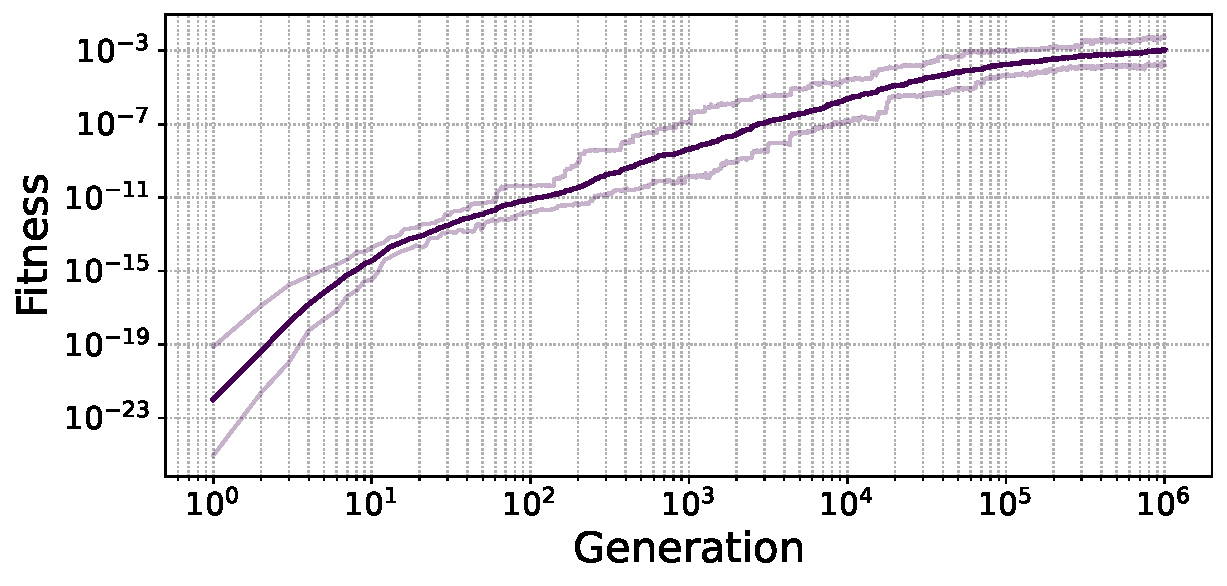
\includegraphics[width=0.75\textwidth]{ploscb/img/all_fitness.pdf}
  %\vspace{0.1cm}
  \caption{Geometric average of the fitness of the best individual in each of the 30 replicates, at every generation.
  Lighter lines represent the first and last decile of the data.}
  \label{fig:main_fitness}
\end{figure}

In our simulations, the fitness of the best individual in each population increases over evolutionary time, as shown in Figure~\ref{fig:main_fitness}, meaning that better and better phenotypes are selected by evolution. More precisely, the expression levels of the genes in individuals in our model therefore evolve towards their respective targets, as defined previously in Section~\ref{sec:evol_model}.

% Example genome in both environments
\begin{figure}[H]
  \centering
  \begin{subfigure}[t]{\textwidth}
    \centering
    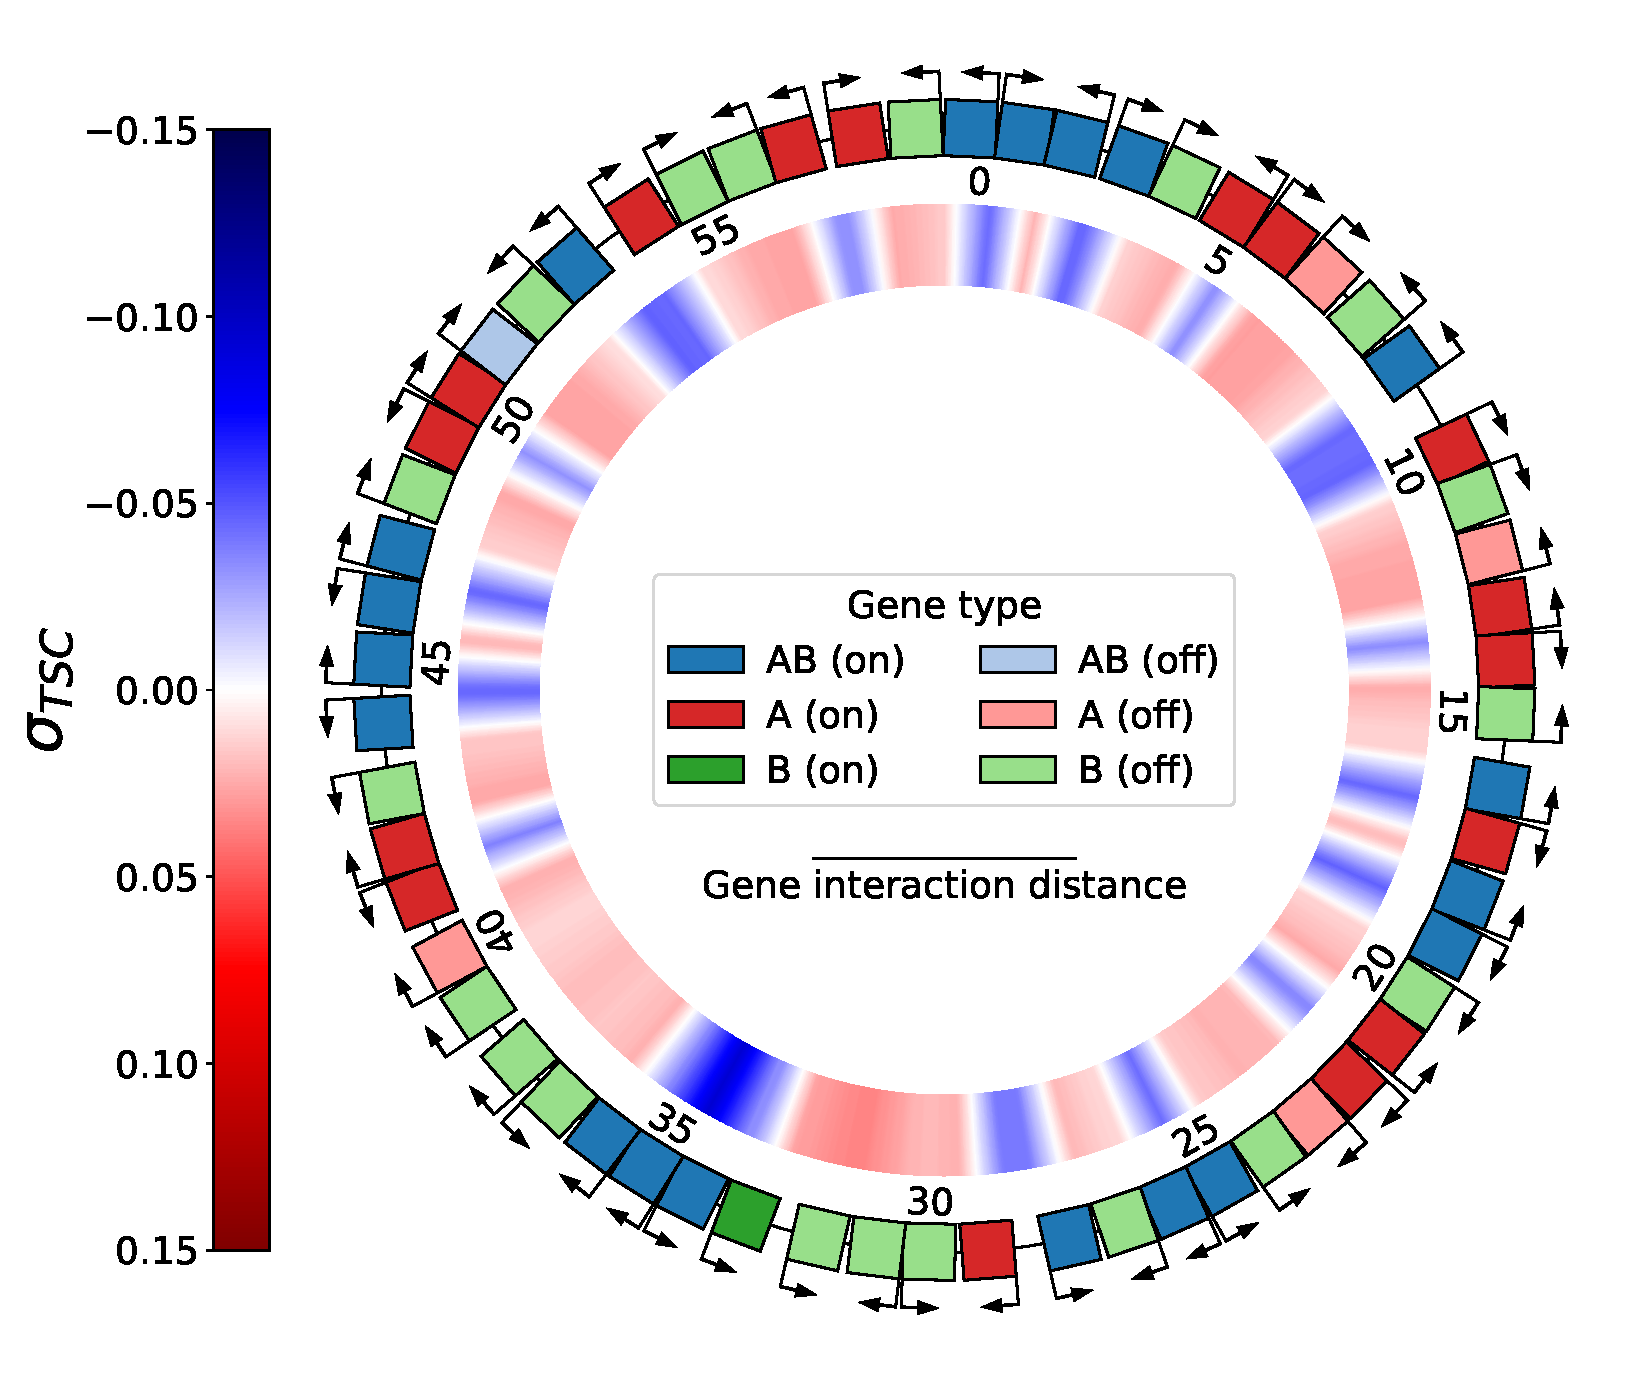
\includegraphics[height=7cm]{ploscb/img/genome_and_tsc_rep21_env_A.pdf}
    \hspace{-0.5cm}
    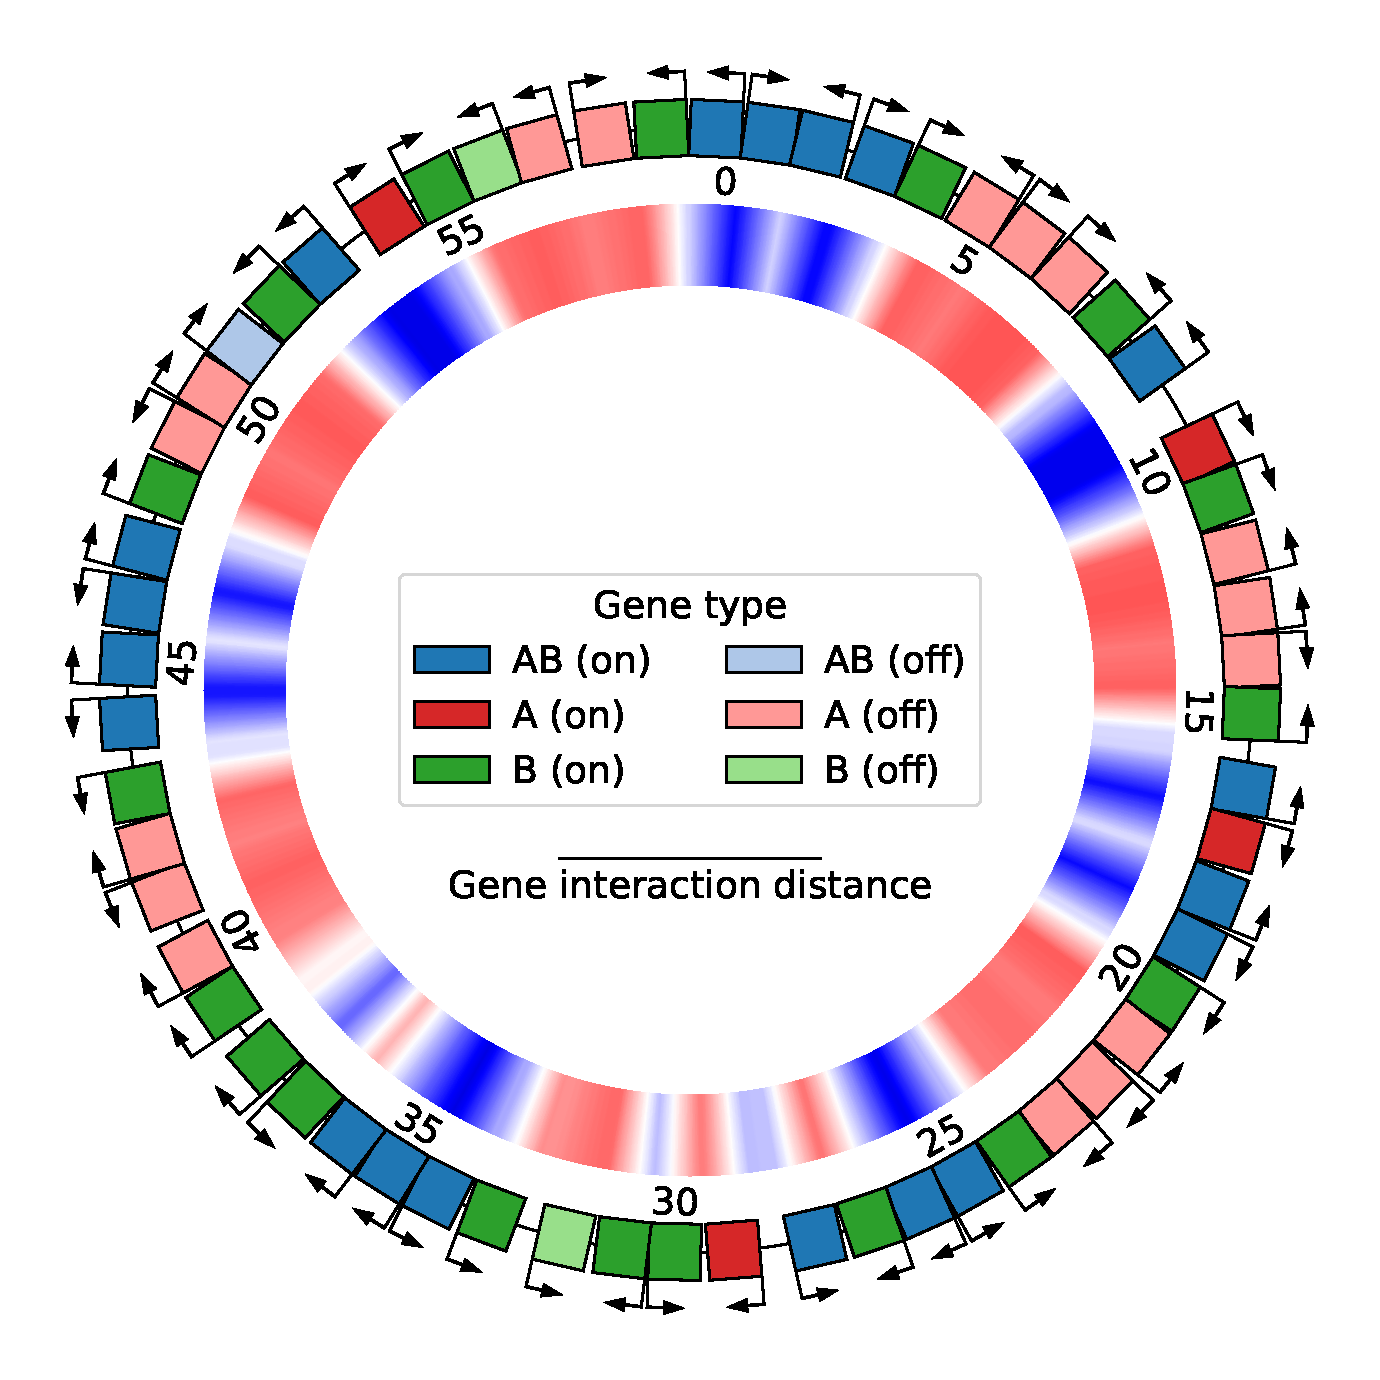
\includegraphics[height=7cm]{ploscb/img/genome_and_tsc_rep21_env_B.pdf}
  \end{subfigure}
  \caption{Genome of the best individual at the last generation of replicate 21, evaluated in environments A (left) and B (right).
  In addition to Figure~\ref{fig:random_indiv}, the outer ring shows the state of each gene: dark color, activated -- light color, inhibited.
  %Genes are numerated clockwise, starting from the top.
  The inner ring shows the level of transcription-generated DNA supercoiling at every position on the genome: Shades of blue represent negative supercoiling, and shades of red positive supercoiling.}
  \label{fig:genomes}
\end{figure}

The genome of an example evolved individual at the end of the simulation is depicted in Figure~\ref{fig:genomes}, in each environment.
Different activation patterns for each gene class are clearly visible on the genome.
Indeed, all \emph{AB} genes except one are activated (dark blue) in each environment in this individual, whereas 19 out of 20 \emph{B} genes are correctly inhibited (light green) in environment A (left) and 18 correctly activated (dark green) in environment B (right).
Conversely, 16 \emph{A} genes are activated in environment A, and 16 inhibited in environment B.

The transcription-generated supercoiling represented in the inner ring furthermore changes consistently with the gene activation patterns between the two environments: red zones, where DNA is positively supercoiled, contain inhibited genes, whereas blue zones, where DNA is negatively supercoiled, contain activated genes.
In this individual, the coupling between supercoiling and transcription therefore generates a steady state of gene expression levels that is consistent with the evolutionary target that was originally set in each environment.

% Evolution of gene _activation_ by gene class
\begin{figure}[H]
  \begin{subfigure}[t]{\textwidth}
    \centering
    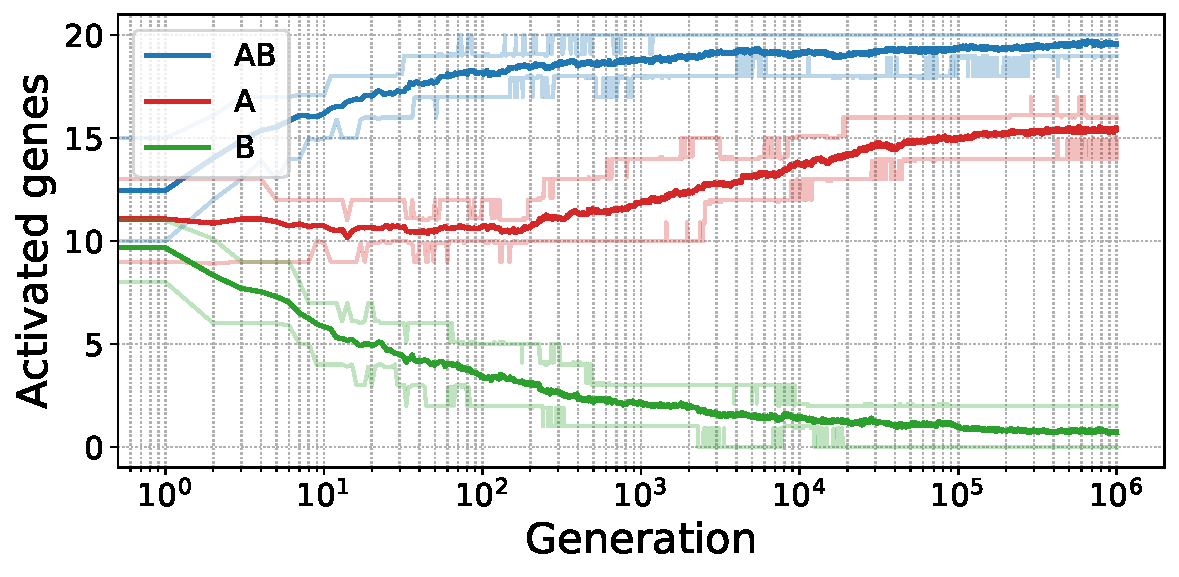
\includegraphics[width=0.75\textwidth]{ploscb/img/gene_activity_env_A_quantile.pdf}
    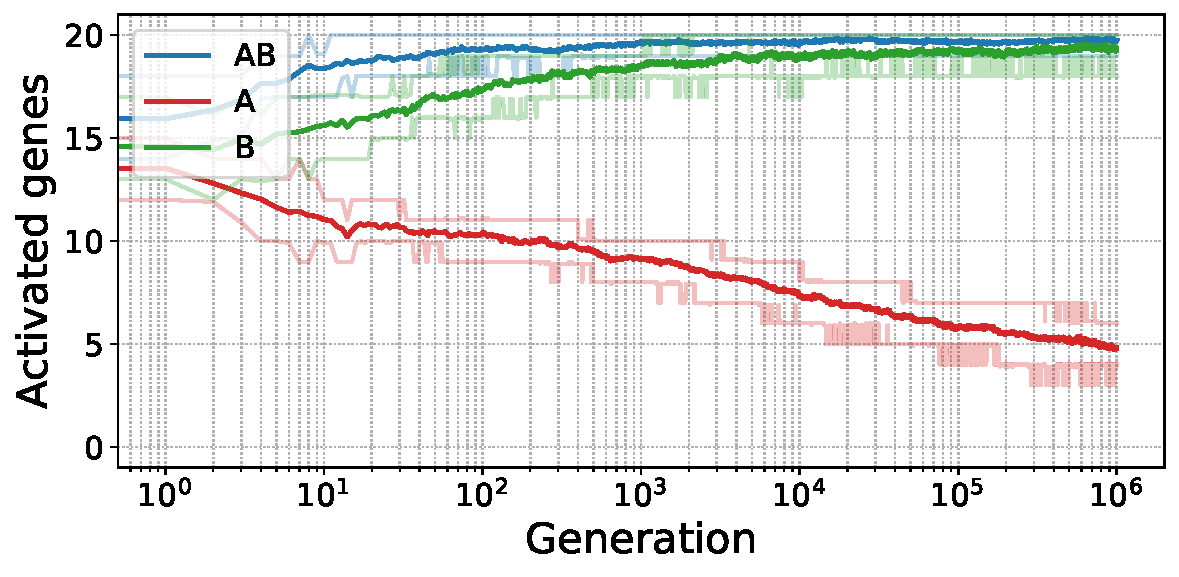
\includegraphics[width=0.75\textwidth]{ploscb/img/gene_activity_env_B_quantile.pdf}
  \end{subfigure}
  \caption{Average number of activated genes (out of 20) of each type in the best individual at every generation, averaged over the 30 replicates, in environments A (top) and B (bottom).
  Lighter lines represent the first and last decile of the data.}
  \label{fig:gene_activity_by_env}
\end{figure}

\paragraph{Evolution of Class-Specific Gene Expression Levels}
These results are however not specific to this particular individual.
Figure~\ref{fig:gene_activity_by_env} shows that, averaging over all replicates, the number of activated genes in each class evolves towards their respective target.
In each environment, the average number of activated \emph{AB} genes quickly reaches nearly 20, its maximum value, as expected from their target; \emph{B} genes follow the same behavior, evolving towards nearly full activation in environment B and nearly full inhibition in environment A.
\emph{A} genes follow a slightly different course, as the number of activated \emph{A} genes seems to converge to approximatively 15 out of the expected 20 in environment A, but continues to decrease towards the expected 0 in environment B by the end of the simulations.
The incomplete match to their target of \emph{A} genes is however not unexpected.
Environment A is indeed characterized by a positive supercoiling shift $\sigma_A > 0$, while environment B is characterized by a negative supercoiling shift $\sigma_B < 0$.
As positive supercoiling lowers promoter activity, it is more difficult for a gene to have a high transcription rate in environment A rather than in environment B.
\emph{A} genes must therefore complete the more difficult task of being activated in the ``hard'' environment A, while being inhibited in the ``easy'' environment B.
Differentiated expression levels therefore evolve in our model for each type of gene, as a result of the different supercoiling levels imposed by the environmental conditions.
These results corroborate the preliminary results in~\citep{grohens2021}, using the more comprehensive model presented in this manuscript.
% which incorporates gene length into the computation of the transcription-supercoiling coupling, and separates promoter activity from gene transcription levels.

% Final message: evolution of hypercoiling-activated phenotype
\begin{figure}[H]
  \centering
  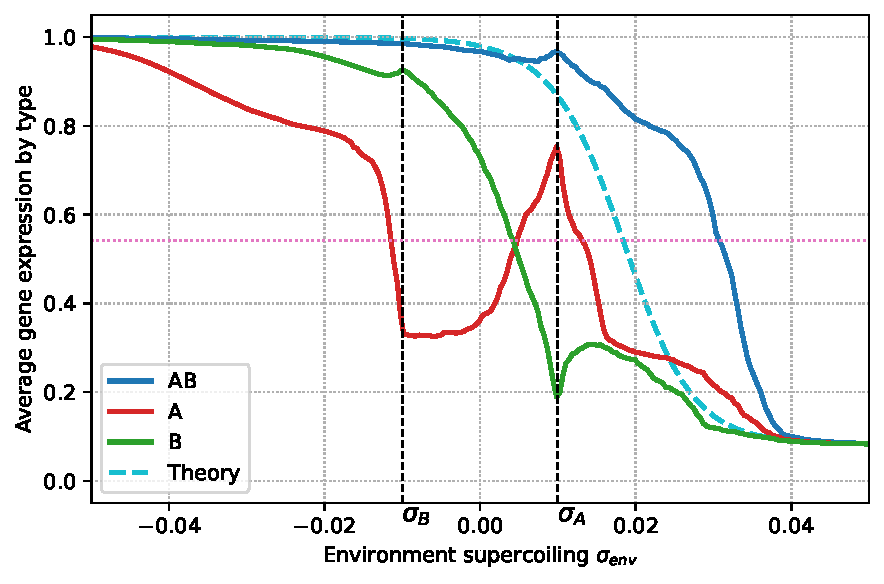
\includegraphics[width=0.75\textwidth]{ploscb/img/activity_sigmas_avg.pdf}
  \caption{Average steady-state gene expression level for each class of gene, as a function of the environmental supercoiling $\sigma_{env}$, averaged over the best individuals of the 30 replicates.
  The cyan line represents the theoretical expression level of a isolated neighbor-less gene for comparison.
  The black vertical lines represent environments A and B, in which individuals evolve during the simulation, and the pink horizontal line marks $e_{1/2}$, the threshold above which a gene is considered active.}
  \label{fig:activity_by_sigma}
\end{figure}

\paragraph{Evolution of Relaxation-Activated Genes}
In our model, the expression level of a gene increases exponentially with the activity of its promoter, which itself increases as a sigmoidal function of negative supercoiling.
When measuring the response of an individual's genes to variation in the environmental supercoiling $\sigma_{env}$, a qualitatively similar response could therefore be expected.

Figure~\ref{fig:activity_by_sigma} however depicts striking differences between the responses of genes of different types to the environment supercoiling level.
Indeed, while \emph{AB} and \emph{B} genes (blue and green curves) display an expression level that decreases as the supercoiling increases, remaining close to the behavior of an isolated gene (cyan curve), \emph{A} genes display a completely different behavior.
These genes show a non-monotonic response to environmental supercoiling, decreasing until a local minimum in expression at $\sigma_B$, then increasing again until a local maximum at $\sigma_A$, before decreasing again like genes of the other classes.
In other words, \emph{A} genes present a phenotype of activation by environmental relaxation of DNA, for values between $\sigma_B$ and $\sigma_A$, even though the promoter activity of an isolated \emph{A} gene decreases with DNA relaxation.

The transcription-supercoiling coupling therefore provides, in our model, a regulatory layer that mediates the transcriptional response to a global variation in DNA supercoiling caused by the environment in a way that allows for the evolution of a opposite response to the one displayed by a non-interacting, neighborless gene.


\subsection{Evolution of Local Genome Organization}

Having characterized the different patterns of gene transcription that evolved in our simulations in response to different environmental conditions, we sought to determine the genome organization patterns that necessarily underlie these patterns, as the only difference between individuals in our model is the relative position and orientation of the genes on their genome.

We started by studying genome organization at the local level, and measured the relative abundance of pairs of neighboring genes in every relative orientation: convergent, divergent, or in tandem.
The relative orientation between neighboring genes determines the mode of interaction between these genes, as described by the twin-domain model of transcription-generated supercoiling: mutual activation for divergent genes, mutual inhibition for convergent genes, and activation (resp. inhibition) of the upstream (resp. downstream) gene by the downstream (resp. upstream) gene.

As the different gene types must evolve different activation patterns in each environment to have a high fitness in the model, we separated the pair counts by the type of each gene in the pair.
Finally, in order to quantify the actual strength of the coupling between these pairs, we measured the total level of positive and negative supercoiling generated by the transcription of each gene in the pair at the promoter of the other gene in the pair.
The results are presented in Figure~\ref{fig:pair_results}, with the left-hand side panel showing the number of pairs of each type, and the right-hand side panel the corresponding transcription-generated supercoiling levels; several patterns markedly emerge from the data.

\begin{figure}[H]
  \centering
  \begin{subfigure}[t]{\textwidth}
    \centering
    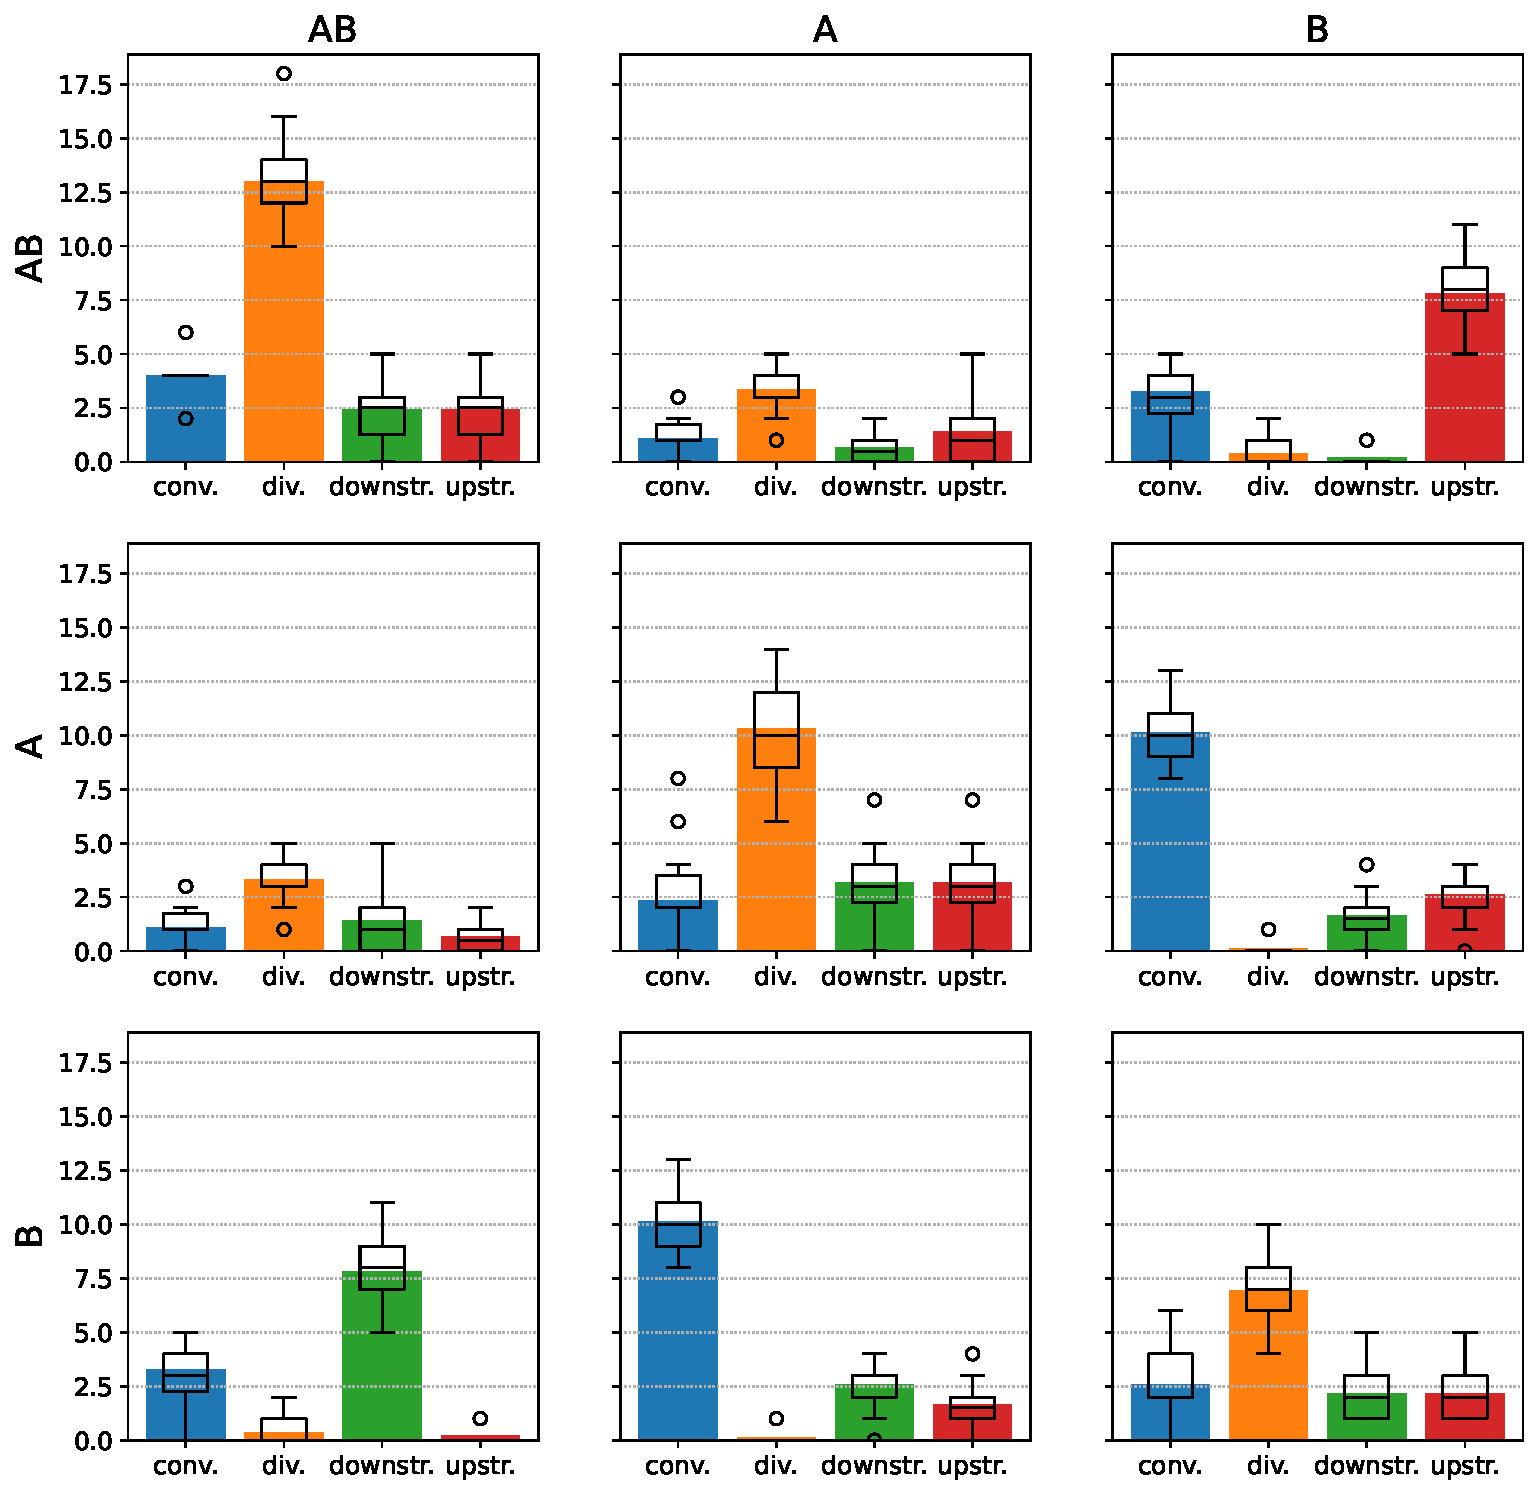
\includegraphics[height=7.3cm]{ploscb/img/gene_pair_counts.pdf}
    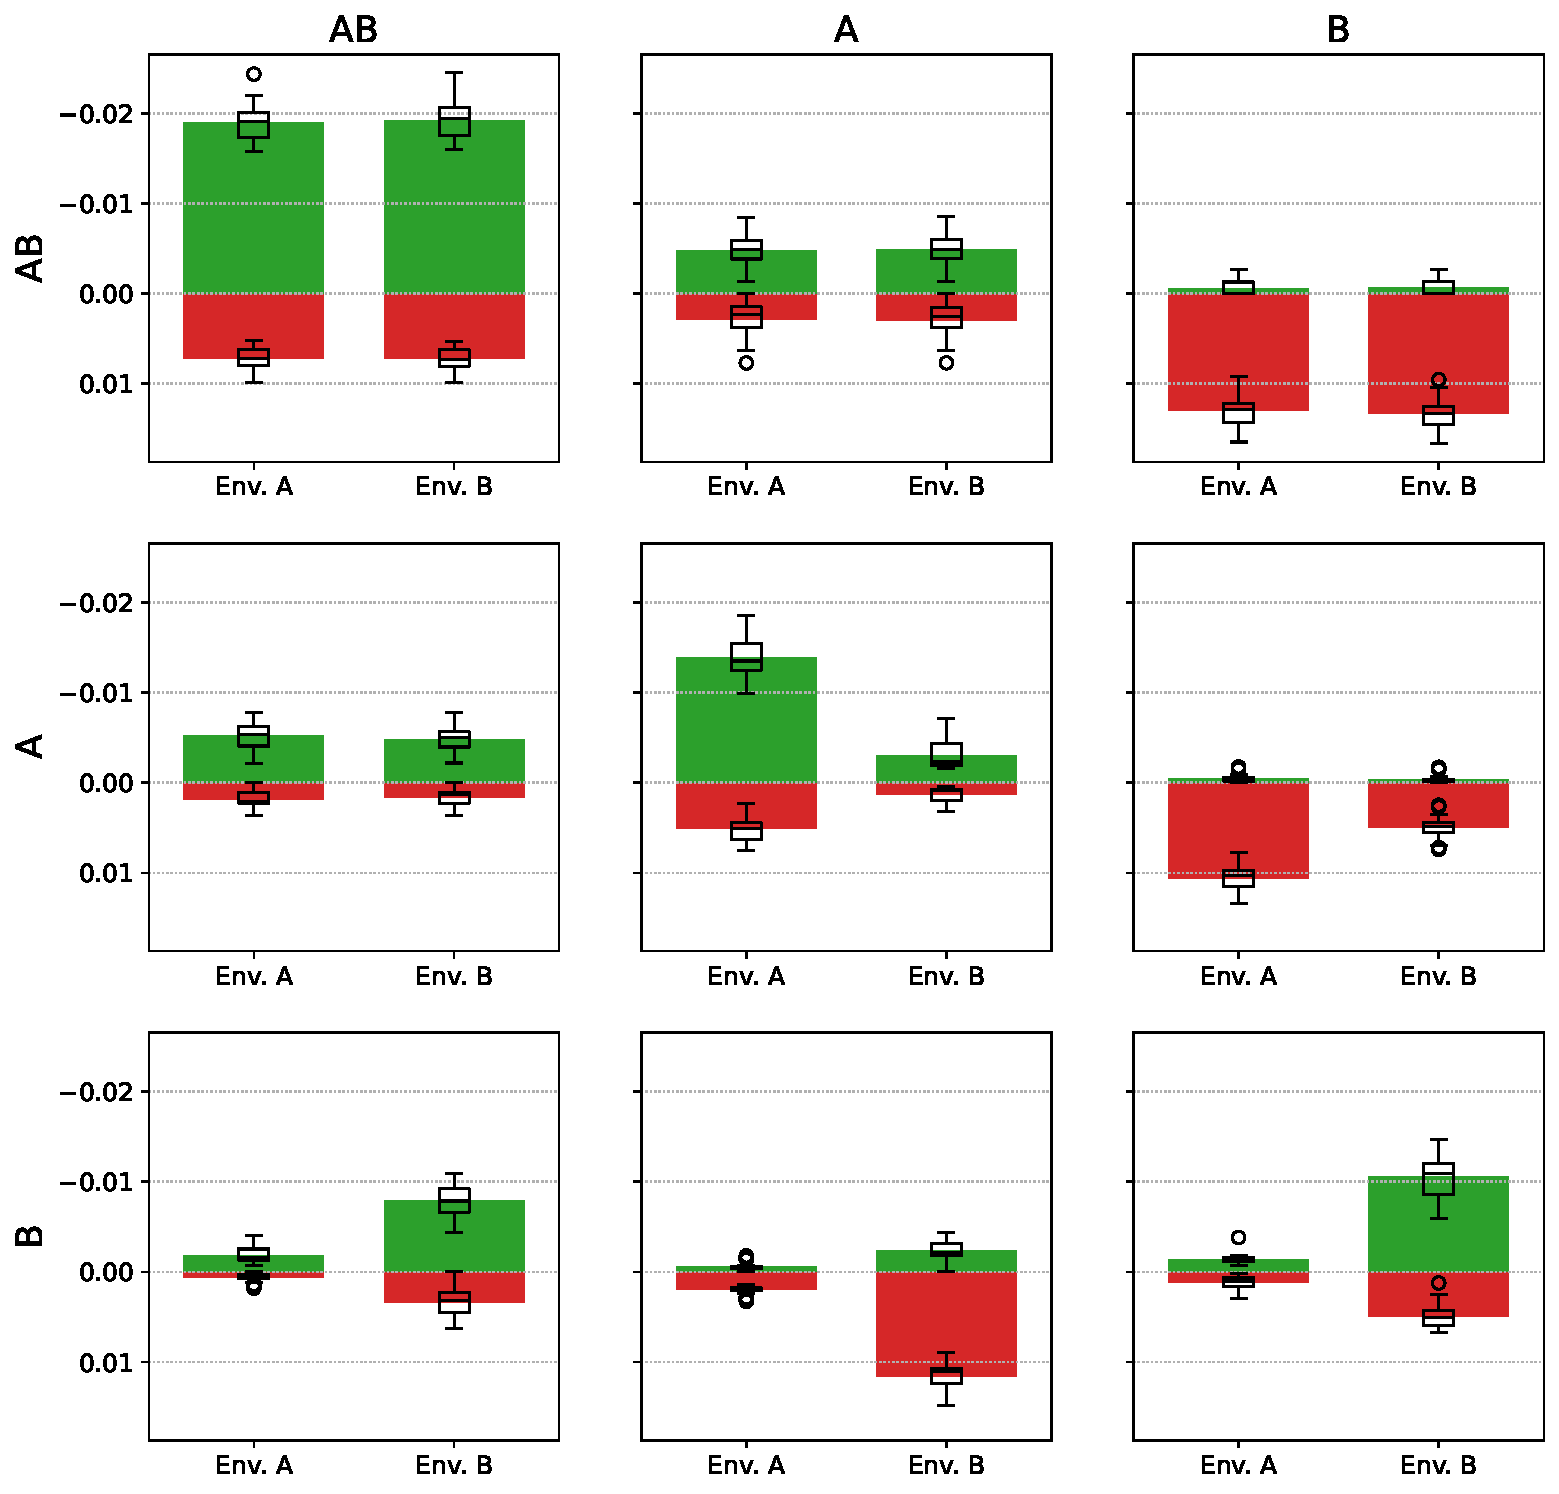
\includegraphics[height=7.3cm]{ploscb/img/pos_neg_supercoiling_pairs.pdf}
  \end{subfigure}
  \caption{Interactions between pairs of neighboring genes.
  The left-hand side panel shows the number of pairs of neighboring genes, split by the type of the first gene (sub-row) and of the second gene (sub-column) in the pair, and by relative orientation (bars in each sub-panel: convergent, divergent, upstream, or downstream).
  As there are 20 genes of each type, and each gene appears in two pairs, the total number of pairs in each sub-row and sub-column is 40.
  The right-hand side panel shows the total amount of positive (red) and negative (green) transcription-generated supercoiling due to each gene type (sub-row) measured at the promoter of each gene type (sub-column), averaged over all genes of that type, in each environment.
  All data is averaged over the best individual of each of the 30 replicates, and box plots indicate the median and dispersion between the replicates.}
  \label{fig:pair_results}
\end{figure}

% Divergent pairs: AB
\paragraph{Genomes Are Enriched in Divergent \emph{AB}/\emph{AB} Pairs}
The most frequent type of gene pair is pairs of divergently oriented \emph{AB} genes.
These pairs make up on average 13 out of 40 pairs containing an \emph{AB} gene (\emph{AB}/\emph{AB} sub-panel on the left-hand side of Figure~\ref{fig:pair_results}), meaning that two-thirds of \emph{AB} genes are part of a divergent pair with another \emph{AB} gene.
These divergent pairs generate an average negative supercoiling of around 0.012, both in environment A and in environment B (summing the positive and negative bars in the \emph{AB}/\emph{AB} sub-panel on the right-hand side of Figure~\ref{fig:pair_results}).
This value is slightly stronger than the environmental supercoiling in absolute value ($|\sigma_A| = |\sigma_B| = 0.01$), showing that the interaction between neighboring genes can generate a variation in supercoiling that is as strong as the environmental supercoiling itself.

% Divergent pairs: A/A and B/B too, but not A/B
Furthermore, genomes also contain divergent \emph{A}/\emph{A} and \emph{B}/\emph{B} gene pairs or divergent, although less frequently than divergent \emph{AB}/\emph{AB} pairs.
These pairs result in weaker interactions: as these genes must be conditionally expressed or inhibited depending on the environment, the positive feedback loop of divergent pairs seems less evolutionarily favorable for \emph{A} or \emph{B} gene pairs than for \emph{AB} gene pairs.
On the contrary, divergent pairs containing one \emph{A} gene and one \emph{B} gene are almost never found, consistently with theoretical expectation, as \emph{A} and \emph{B} genes should never be expressed in the same environment.

We therefore observe that the local organization of the genome in divergent \emph{AB}/\emph{AB} gene pairs is favored by evolution, as this pattern allows for a high expression of these genes in both environments, but that divergent \emph{A}/\emph{B} gene gene pairs, which would lead to poor fitness, are oppositely seldom found.

% Convergent pairs: A and B, mostly
\paragraph{Genomes are Enriched in Convergent \emph{A}/\emph{B} Pairs}
The pattern in which \emph{B} genes appear most frequently (resp. \emph{A} genes nearly most frequently, just after divergent \emph{A}/\emph{A} pairs) is in convergent pairs with \emph{A} (resp. \emph{B}) genes.
In this case, each gene in the pair theoretically down-regulates the other gene in the pair.
In environment A (resp. B), \emph{A} (resp. \emph{B}) genes indeed generate an average supercoiling variation of 0.01 on \emph{B}  (resp. \emph{A}) genes, a value that is once again comparable to the environmental change in supercoiling (remember that positive supercoiling diminishes gene activity).
This effect is in each case much weaker in the other environment: for example, \emph{A} genes do not inhibit \emph{B} genes in environment B, as they are are much less expressed in this environment, and as the generated supercoiling is directly proportional to the transcription level.

We therefore observe that the local organization of the genome into pairs of convergent \emph{A} and \emph{B} genes that form bistable toggle switches, in which one of the genes in the pair strongly inhibits the other gene in the pair, is also favored by evolution in order to produce differentiated expression levels depending on the environment.

% Talk about AB inhibitors (not interesting)
%Inhibitory interactions are also found in \emph{AB} genes, which are also frequently found upstream of \emph{B} genes: the supercoiling contribution of \emph{AB} genes on \emph{B} genes is strongly positive, in each environment.

% Extend to all pairs of genes
%We can extend our analysis to include all pairs of genes close enough to interact through the transcription-supercoiling coupling (note that this is not a superset of the set of pairs of neighboring genes, as some genes could be neighbors but too far from each other to interact), as depicted in the bottom panels of Figure~\ref{fig:pair_results}.
%Under this light, our qualitative results on the regulatory role of each gene type remains the same: \emph{AB} genes strongly self-activate, as reflected in the high number of divergent pairs, and down-regulate \emph{B} genes; \emph{A} genes and \emph{B} genes strongly down-regulate each other, in the respective environment in which they are highly expressed.

% Global conclusion of this subsection

\subsection{Pairwise Interactions Do Not Recapitulate the Regulatory Network}

In order to understand the extent to which the gene regulatory network generated by the transcription-supercoiling coupling can be summarized by the local organization into pairs that we just described, we systematically studied the behavior of subnetworks of neighboring genes of increasing sizes.

For every odd size $k$ between 1 and the genome size, and for every gene on the genome, we extracted the subnetwork of size $k$ centered around that gene.
Then, we computed the steady-state expression level of every gene in the subnetwork, as for a complete genome, in each environment.
This allowed us to compute the minimum subnetwork size at which a gene has the same activation state as in the complete genome, which is an indicator of the complexity of the interaction network necessary to produce the activation state of that gene.
Two representative examples are presented in Figure~\ref{fig:subnetwork_examples}, and the complete results are shown in Figure~\ref{fig:min_subnetwork}.

\begin{figure}[H]
  \centering
  \begin{subfigure}[t]{\textwidth}
    \centering
    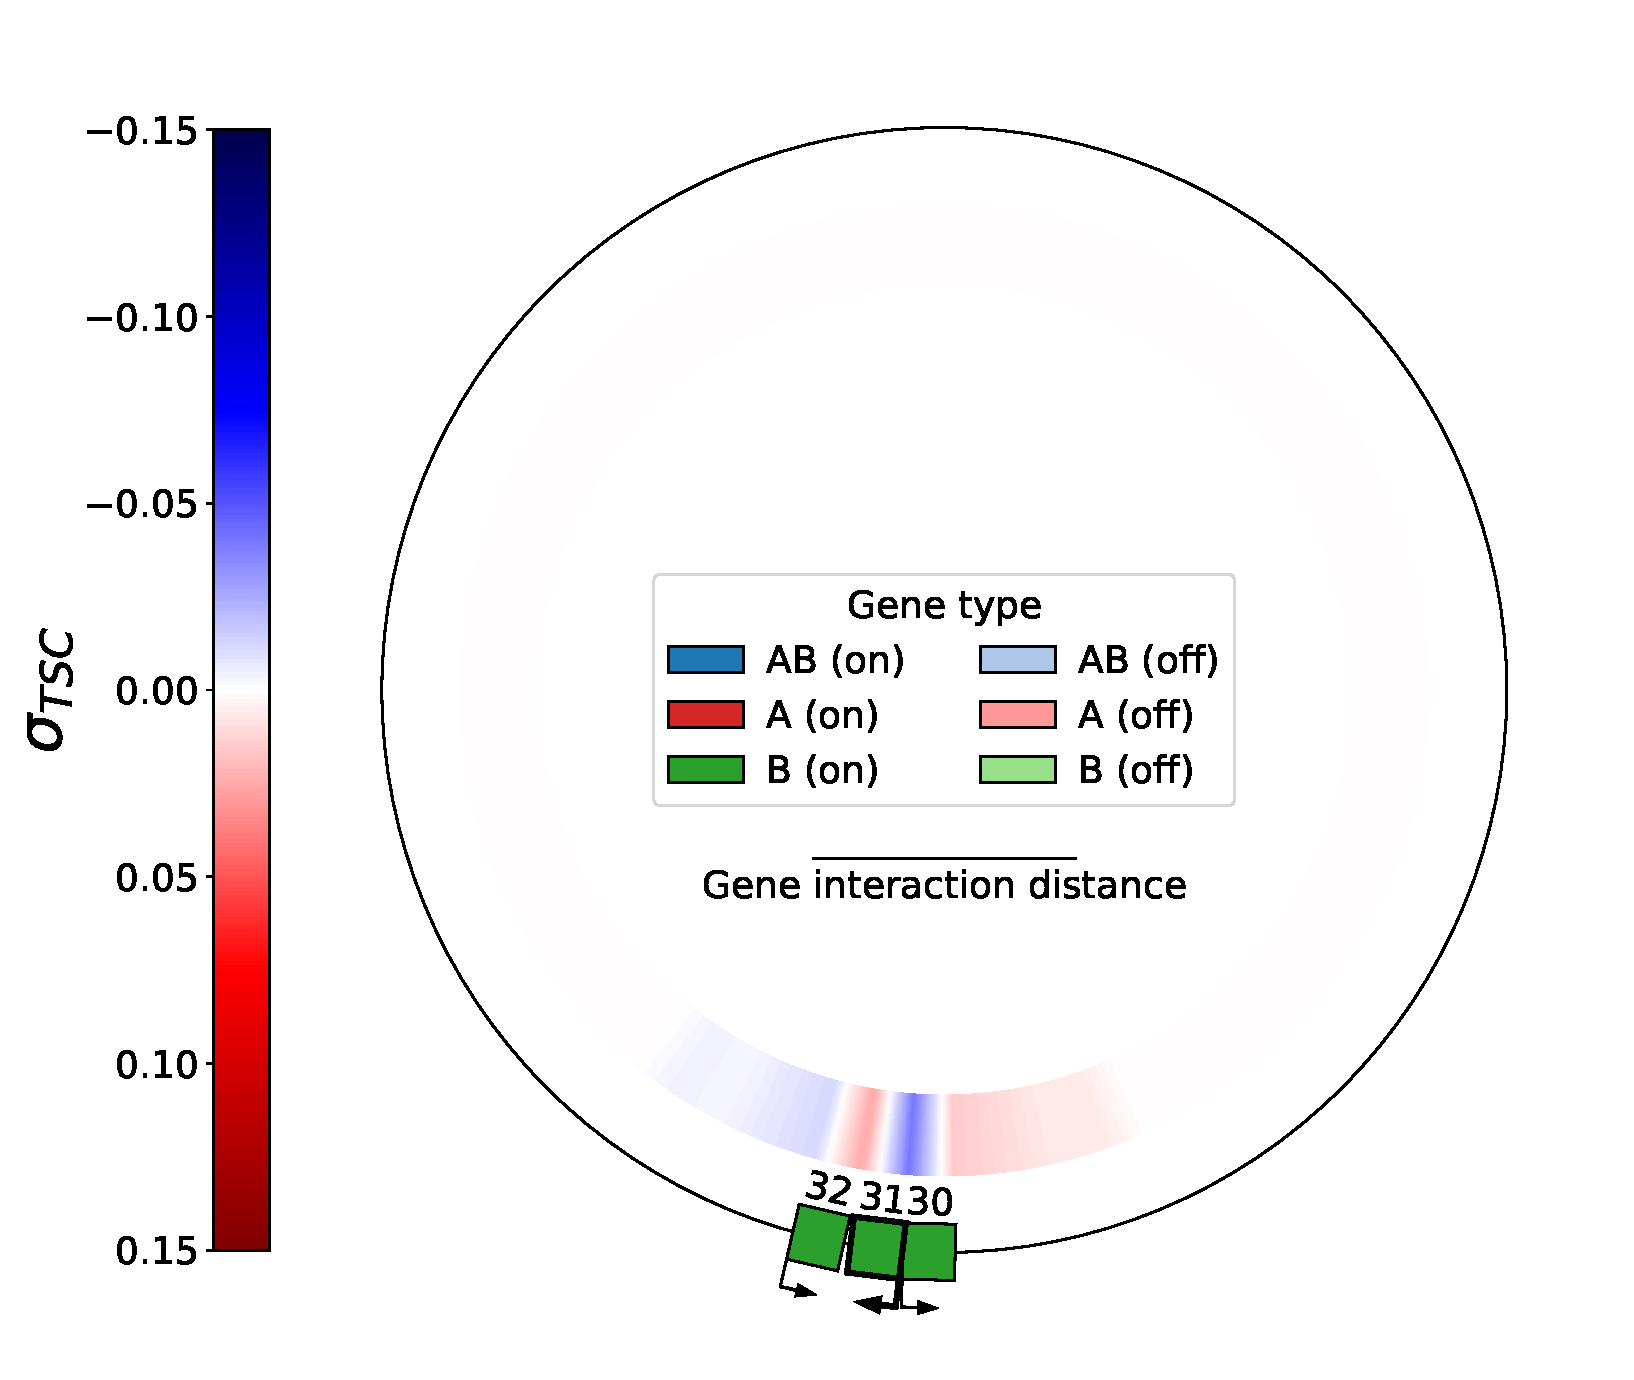
\includegraphics[height=7cm]{ploscb/img/sub_3_genes_30_env_A.pdf}
    \hspace{-0.5cm}
    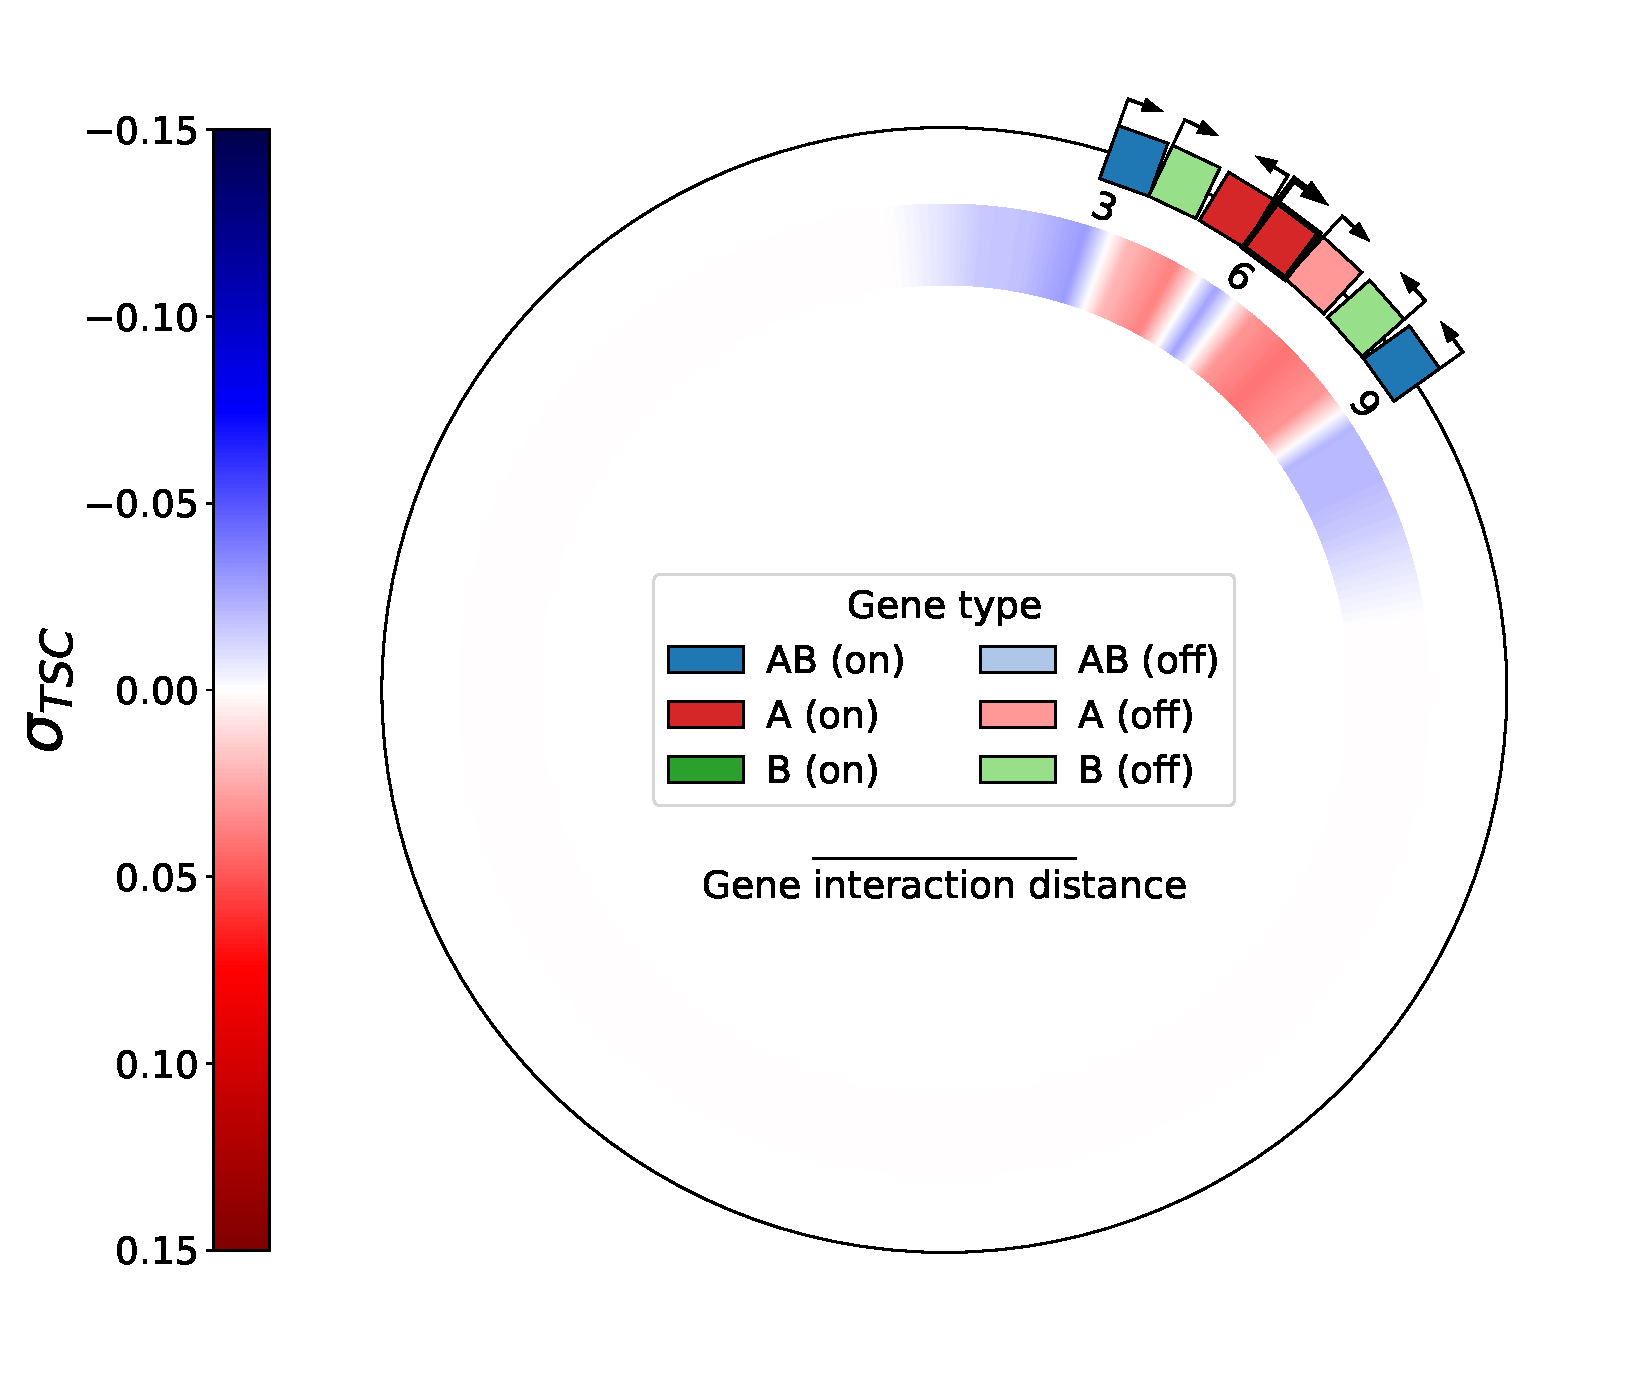
\includegraphics[height=7cm]{ploscb/img/sub_7_genes_03_env_B.pdf}
  \end{subfigure}

  \begin{subfigure}[t]{\textwidth}
    \centering
    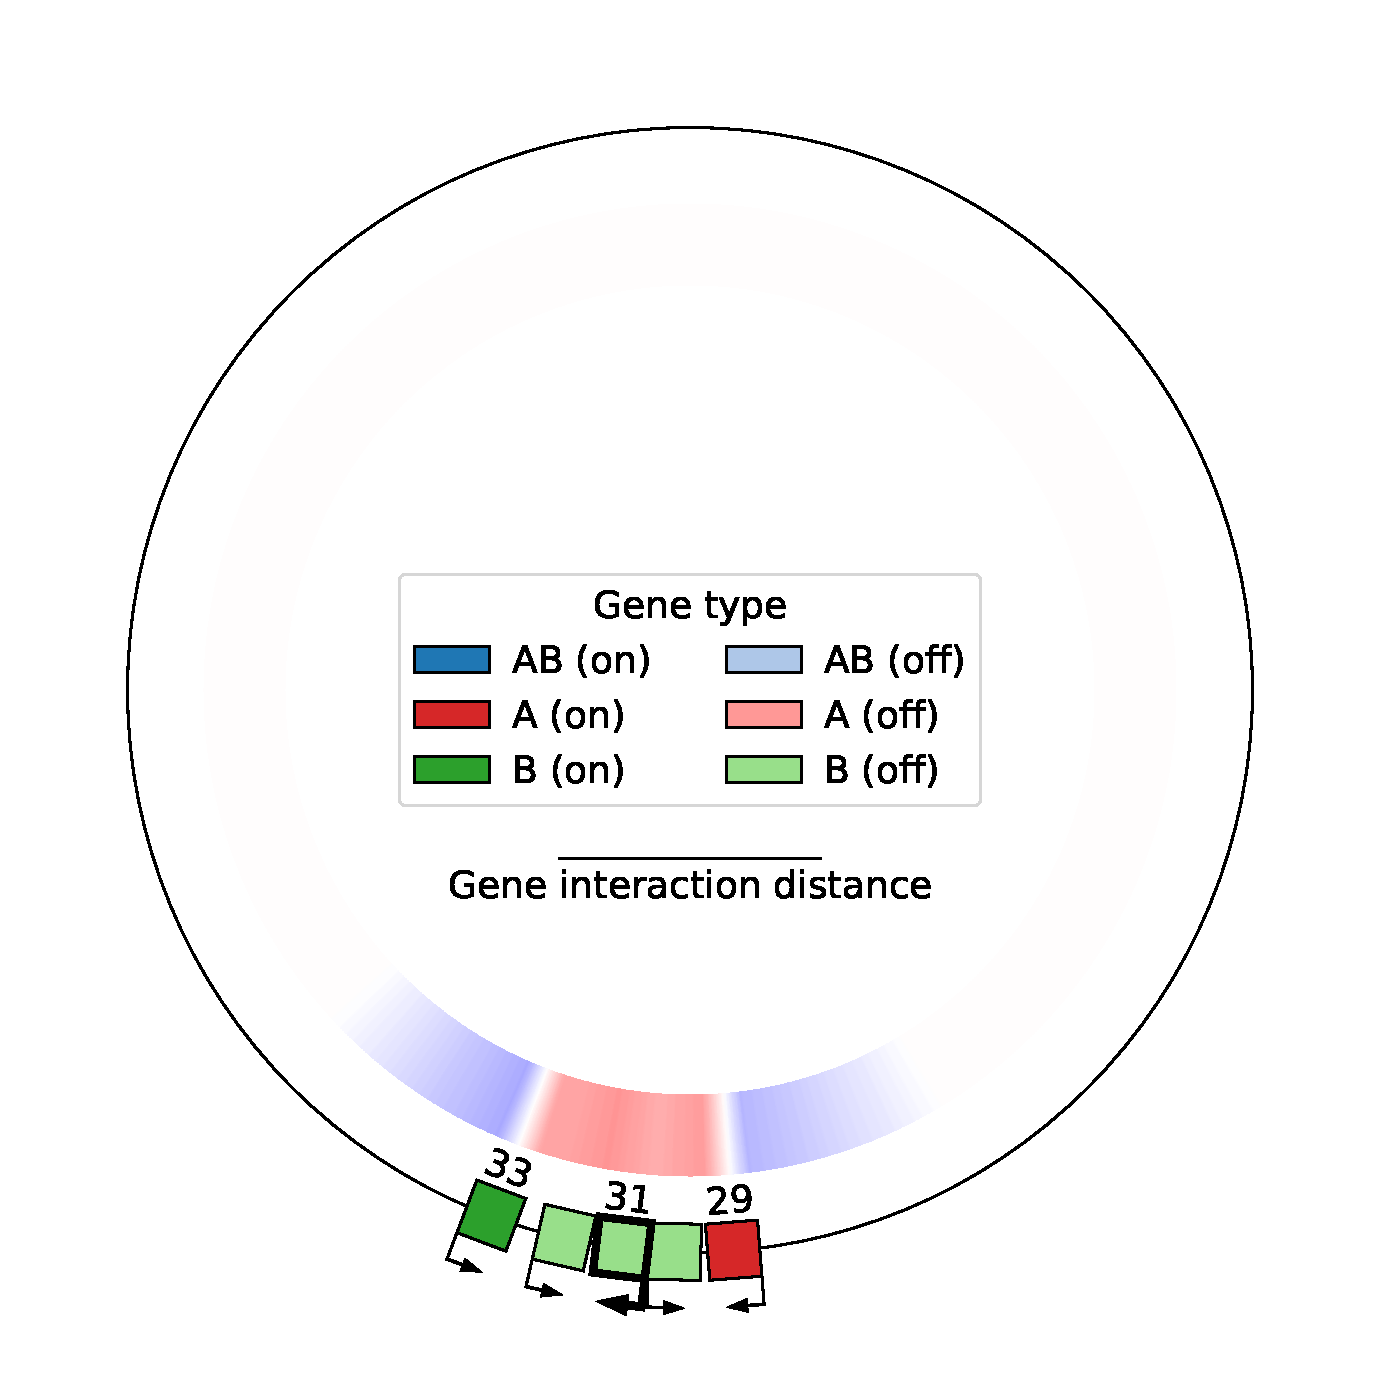
\includegraphics[height=7cm]{ploscb/img/sub_5_genes_29_env_A.pdf}
    \hspace{-0.5cm}
    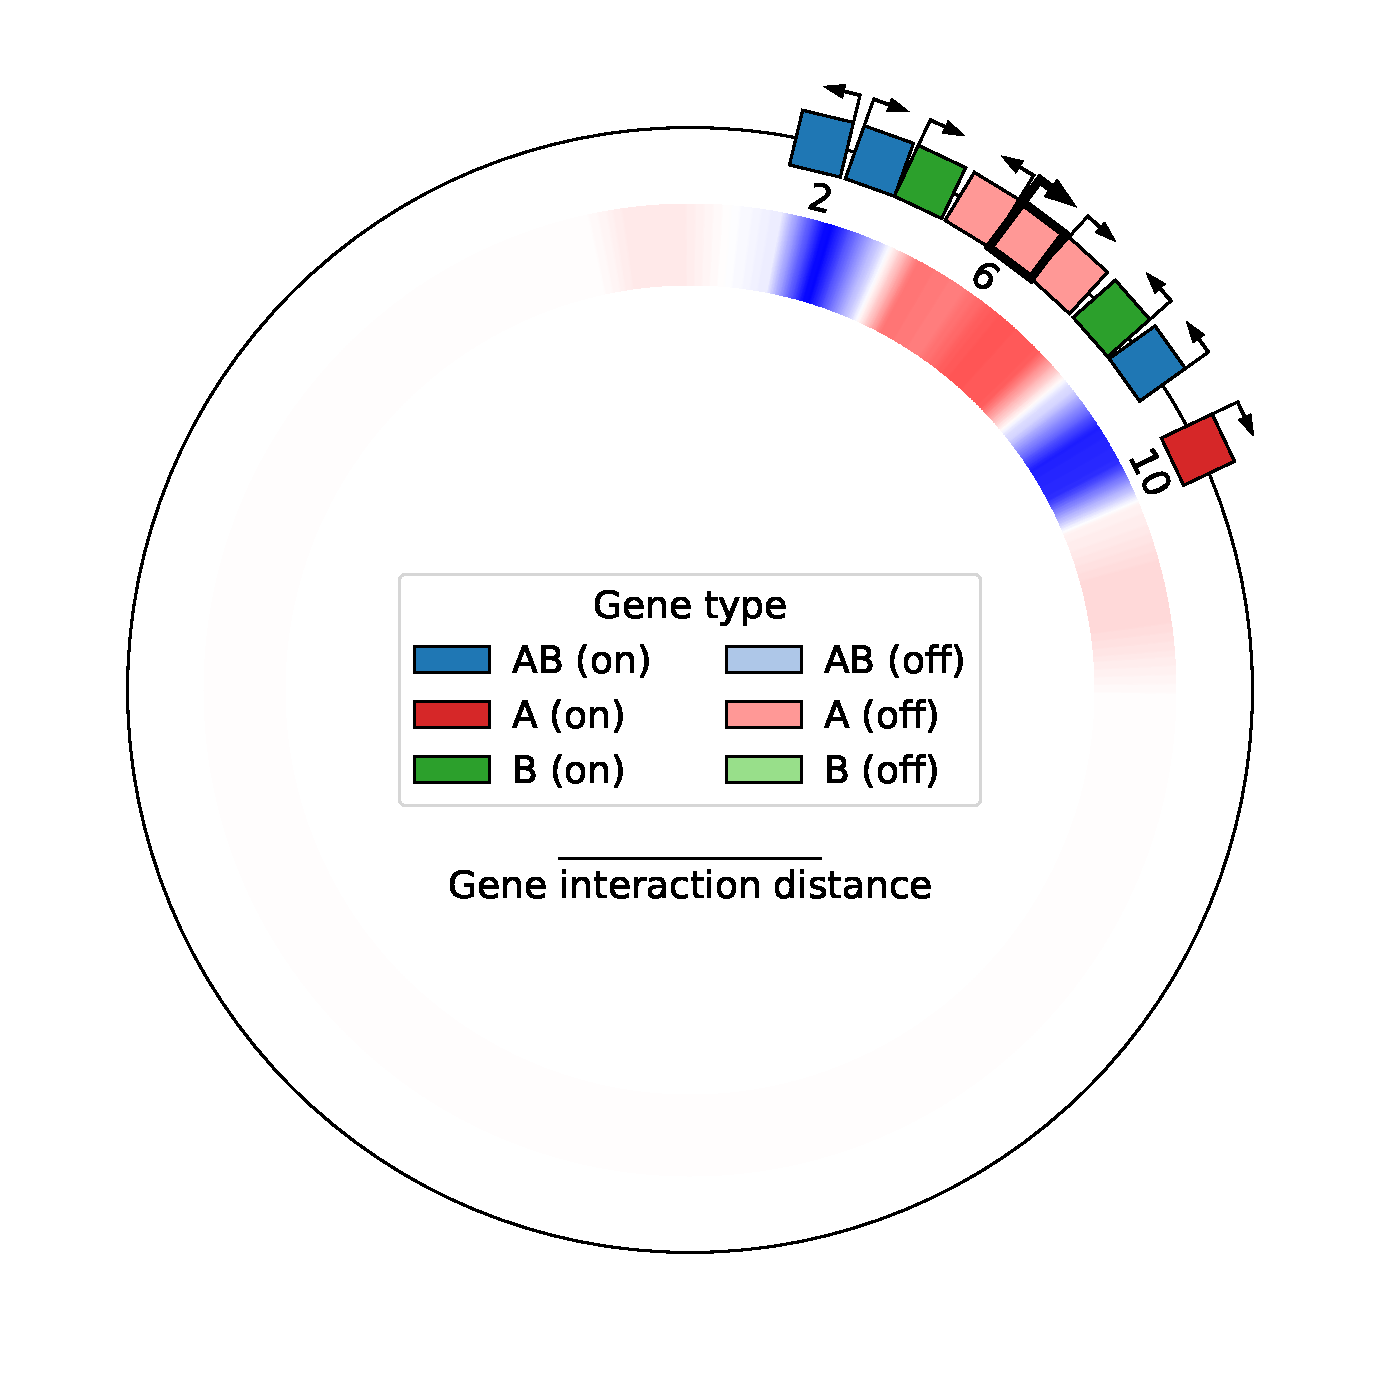
\includegraphics[height=7cm]{ploscb/img/sub_9_genes_02_env_B.pdf}
  \end{subfigure}
  \caption{Left: subnetworks of size 3 (top) and 5 (bottom) centered around gene 31, of type \emph{B}, of the best individual at the end of replicate 21, evaluated in environment A.
  Right: subnetworks of size 7 (top) and 9 (bottom), centered around gene 6, of type \emph{A}, of the same individual, evaluated in environment B.
  In each column, the central gene is correctly inhibited only in the larger subnetwork in the bottom row, but activated in the smaller subnetwork in the top row.}
  \label{fig:subnetwork_examples}
\end{figure}

Figure~\ref{fig:subnetwork_examples} depicts the subnetworks that are needed in order to obtain the inhibition of a representative gene of type \emph{A} in environment B, and of a representative gene of type \emph{B} in environment A, taken from the genome of an evolved individual.
We chose these genes as the minimal subnetwork size needed to inhibit them is close to the mean of the respective distributions presented in Figure~\ref{fig:min_subnetwork}, with a minimal subnetwork size of 9 in the first case and of 5 in the second.
For each gene, the top row represents a subnetwork that is too small to obtain the inhibition of the central gene, and the bottom row represents the subnetwork that actually inhibits the gene.

In each case, increasing the size of the subnetwork by two (or one gene on each side) completely changes the steady state of gene expression levels, and the associated level of transcription-generated supercoiling.
Indeed, on the left-hand side, all 3 genes in the small subnetwork switch states when evaluated inside the larger subnetwork, and on the right-hand side, the two \emph{B} genes and two out of the three central \emph{A} genes switch activation states from the small to the large subnetwork.
In these examples, the activity of a gene is therefore not only dependent on its closest neighbors, but on a larger section of the genome.

\begin{figure}[H]
  \centering
  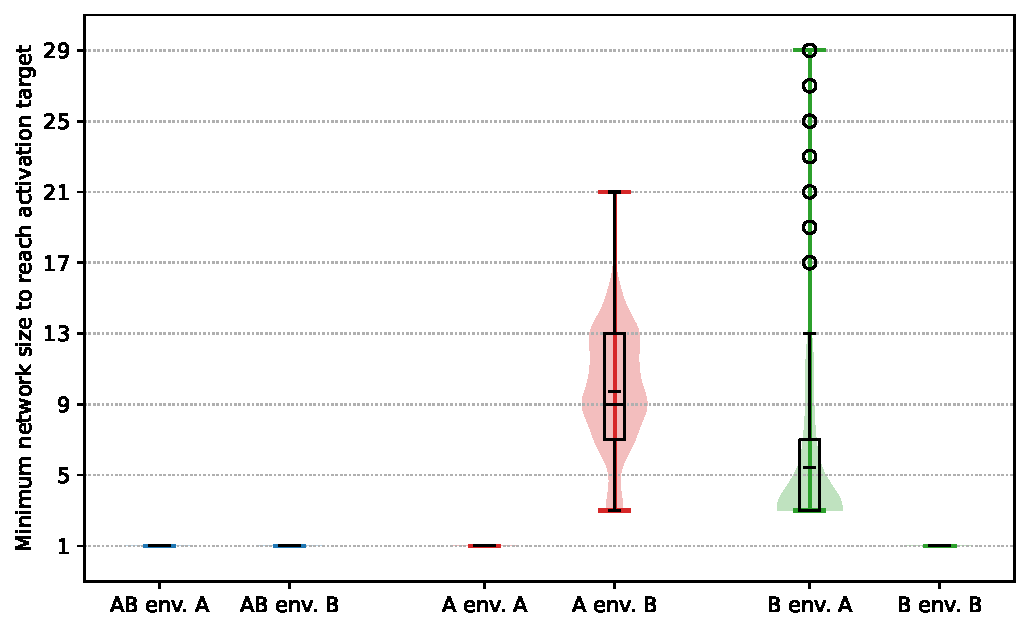
\includegraphics[width=0.75\textwidth]{ploscb/img/min_network_size.pdf}
  \caption{Minimal contiguous subnetwork size needed for the central gene in the subnetwork to have the same activation state as in the complete genome, for each gene type, and in each environment.
  In each case, a box plot showing quartiles and fliers is overlaid on a violin plot representing the whole distribution, and the mean is represented by a smaller tick.
  The data is computed only for genes which present the correct activation state in both environments, which represents 97,7\% of \emph{AB} genes, 92,7\% of \emph{B} genes and 53,2 \% of \emph{A} genes.}
  \label{fig:min_subnetwork}
\end{figure}

Averaging this data over every gene that presents the correct activation state in each environment in the best individual of every replicate, very different patterns appear, depending on whether the targeted behavior for the gene is activation or inhibition, as shown on Figure~\ref{fig:min_subnetwork}.
Remember that, using \emph{E. coli}-inspired parameter values, an isolated gene (corresponding to a subnetwork size of 1) is always activated, because the basal supercoiling level is negative in both environments (as shown in Figure~\ref{fig:activity_by_sigma}).
For \emph{AB} genes in both environments, as well as for \emph{A} genes in environment A and \emph{B} genes in environment B, the experimentally obtained minimum subnetwork size is thus, as expected, of 1.

When the gene activation target is inhibition, that is for \emph{A} genes in environment B and \emph{B} genes in environment A, the picture is however quite different.
In this case, a significantly larger subnetwork is needed in order to obtain inhibition of the central gene: the median subnetwork size is 9 (or 4 genes on each side) for A genes.
For B genes, the median size is 3 (or 1 gene on each side) and the last quartile 7 (or at least 3 genes on each side), with outliers ranging up to a subnetwork size of 29, or nearly half of the whole genome.

The gene regulatory networks evolved through the transcription-supercoiling coupling therefore exhibit a structure that is not always summarized by the local interactions between neighboring genes, but that can on the contrary span a range that is comparable to the size of the whole genome.


\subsection{A Globally Coupled Gene Regulatory Network}

The interaction matrix defined in Section~\ref{sec:indiv_model} provides a natural graph of the interactions between the genes in the genome of an individual.
However, as the effective impact of a gene on other genes through the transcription-supercoiling coupling depends on the transcription level of that gene, this theoretical graph provides an inaccurate picture of the gene interactions that take place at the steady state of gene expression levels.
In order to characterize more finely the gene regulatory networks that evolve in our simulation, we thus constructed another graph, the effective interaction graph, using gene knock-outs.

\begin{figure}[H]
  \centering
  \begin{subfigure}[t]{\textwidth}
    \centering
    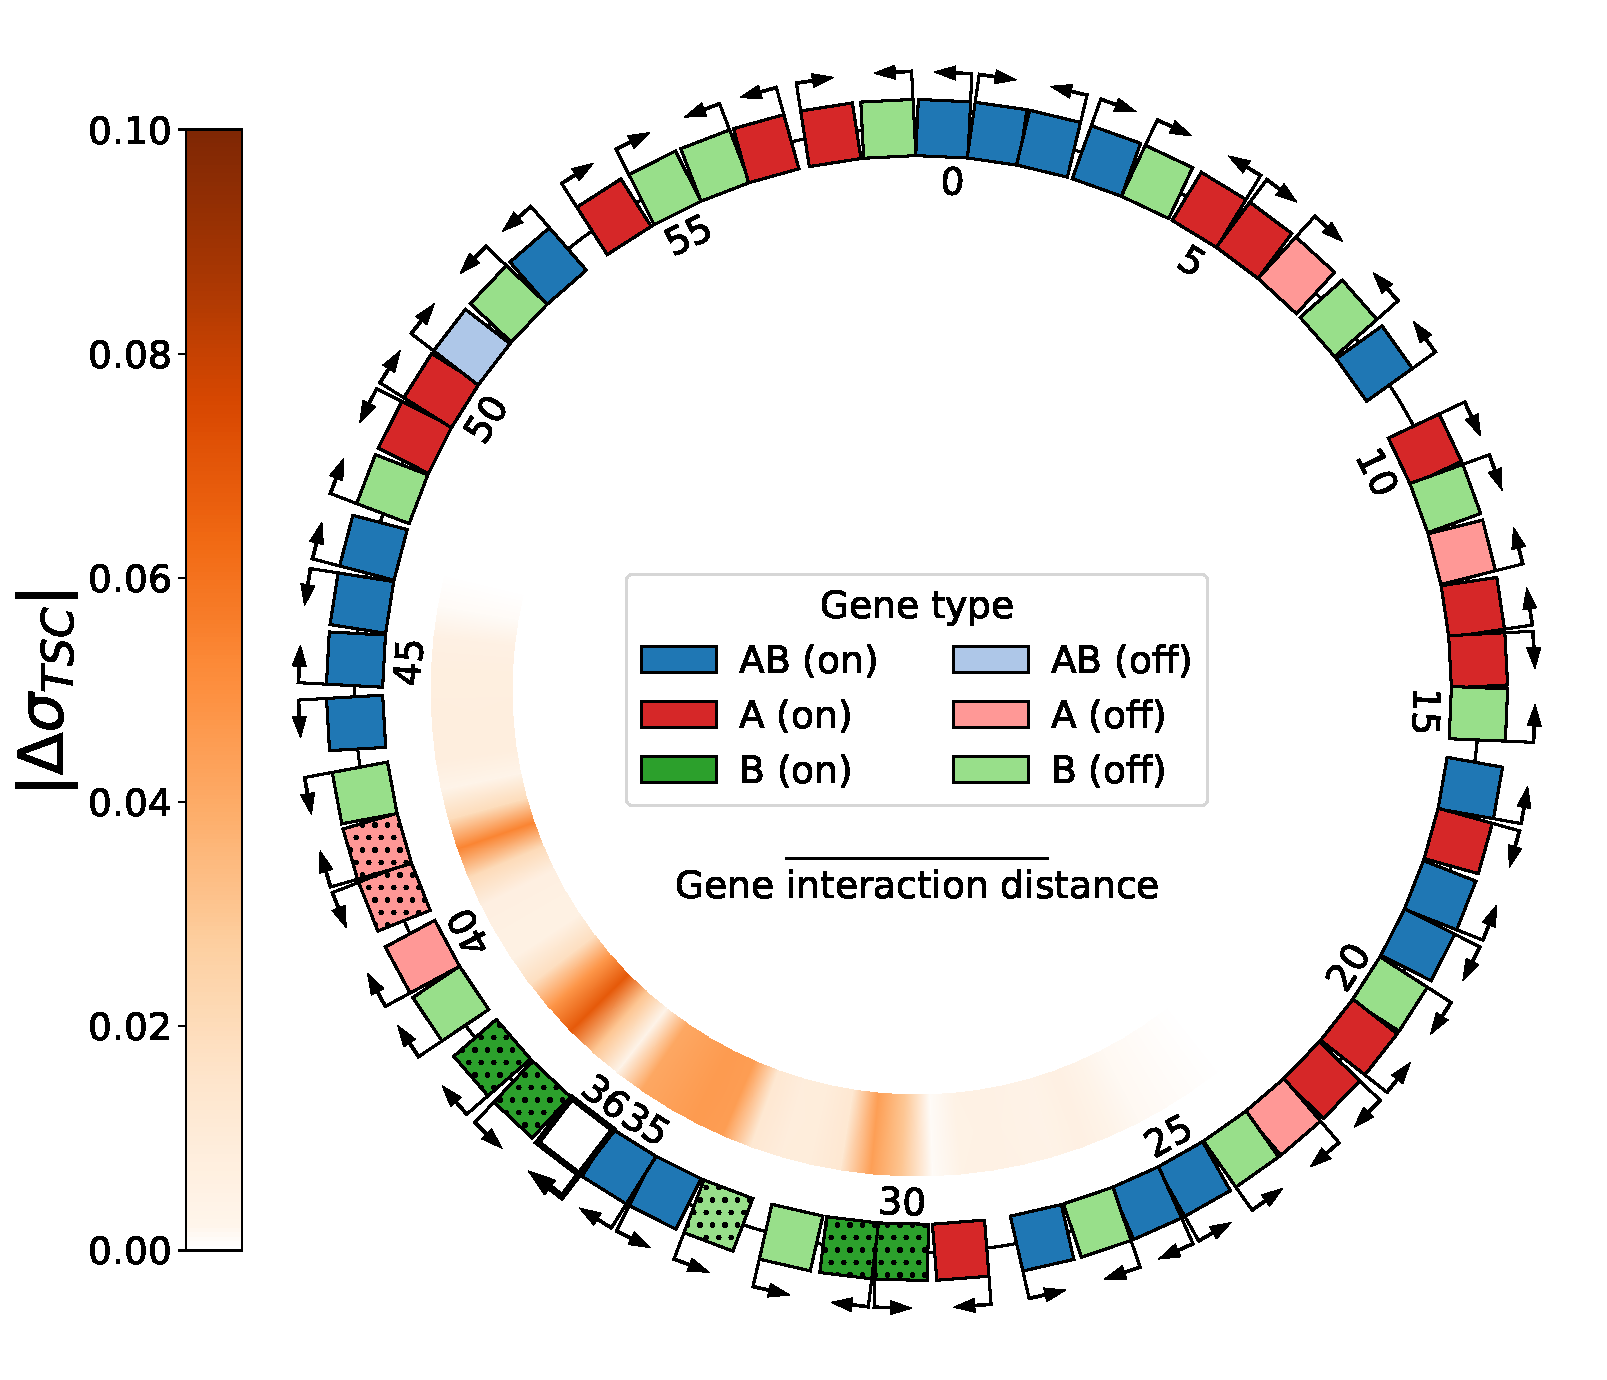
\includegraphics[height=7cm]{ploscb/img/ko_genome_and_tsc_env_A_gene_36.pdf}
    \hspace{-0.5cm}
    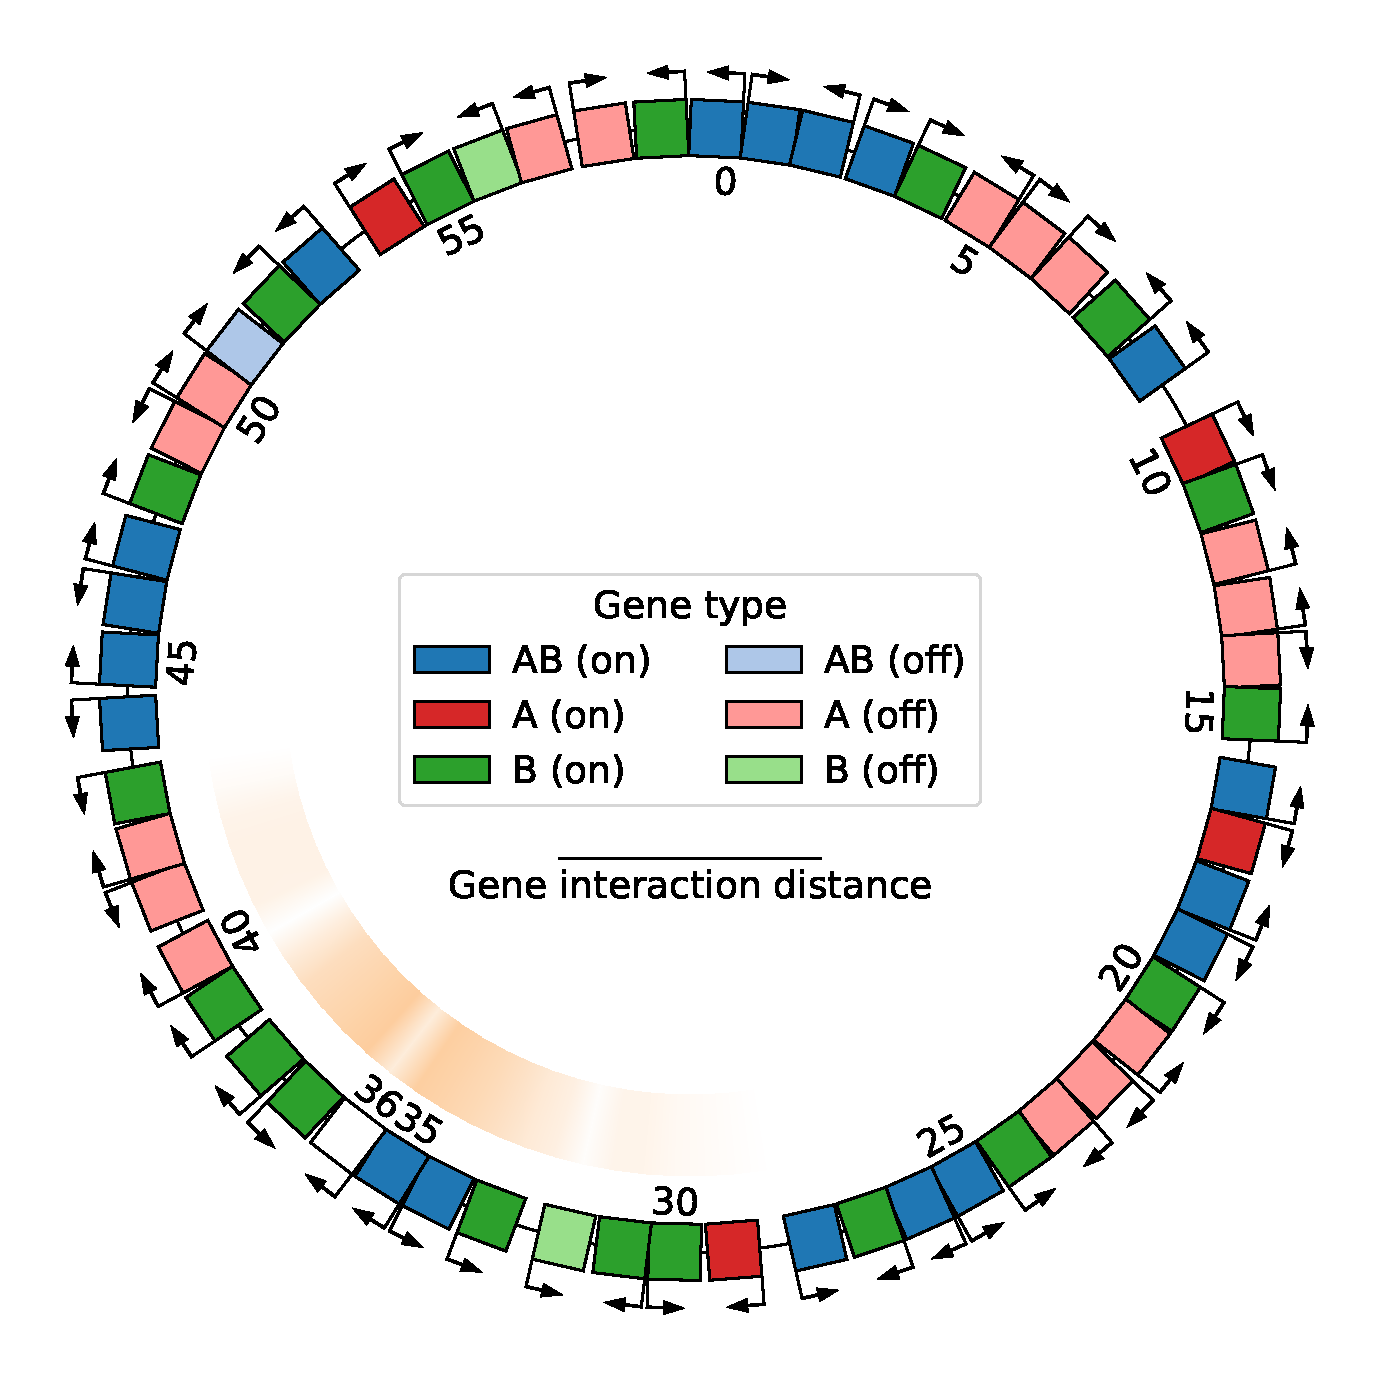
\includegraphics[height=7cm]{ploscb/img/ko_genome_and_tsc_env_B_gene_36.pdf}
  \end{subfigure}
  \caption{Knock-out of gene 36 (in white) of the best individual at the end of replicate 21, evaluated in environments A (left) and B (right).
  Dotted genes represent genes whose activation state was switched by the knockout compared to their state in the original genome.
  The inner ring represents the absolute difference in the level of local supercoiling between the knockout genome and the original genome.}
  \label{fig:ko_genomes}
\end{figure}

\paragraph{Gene Knock-Outs}
To compute the gene transcription rates in an individual with a knocked-out gene, we simply set the transcription rate of the knocked-out gene to zero at every step of the fixed point computation, virtually removing this gene from the genome, but keeping intergenic distances intact.
The result of such a knockout on the genome of an evolved individual is shown in Figure~\ref{fig:ko_genomes}.
The knocked-out gene is gene 36, which is of type \emph{AB} and originally activated in both environments (Figure~\ref{fig:genomes} shows the original genome).
We can see that, in environment A, knocking-out this gene resulted in a switch of the activation state for 7 genes (the hatched genes in the left-hand side of Figure~\ref{fig:ko_genomes}), that are not all contiguously located, and in local supercoiling changes that propagate to the bottom left quarter of the genome; in environment B, knocking-out this gene results in milder supercoiling changes that do not lead to any genes switching state.
In evolved genomes, knocking out even a single gene can therefore lead to a different final state for an important part of the genome.

\begin{figure}[H]
  \centering
  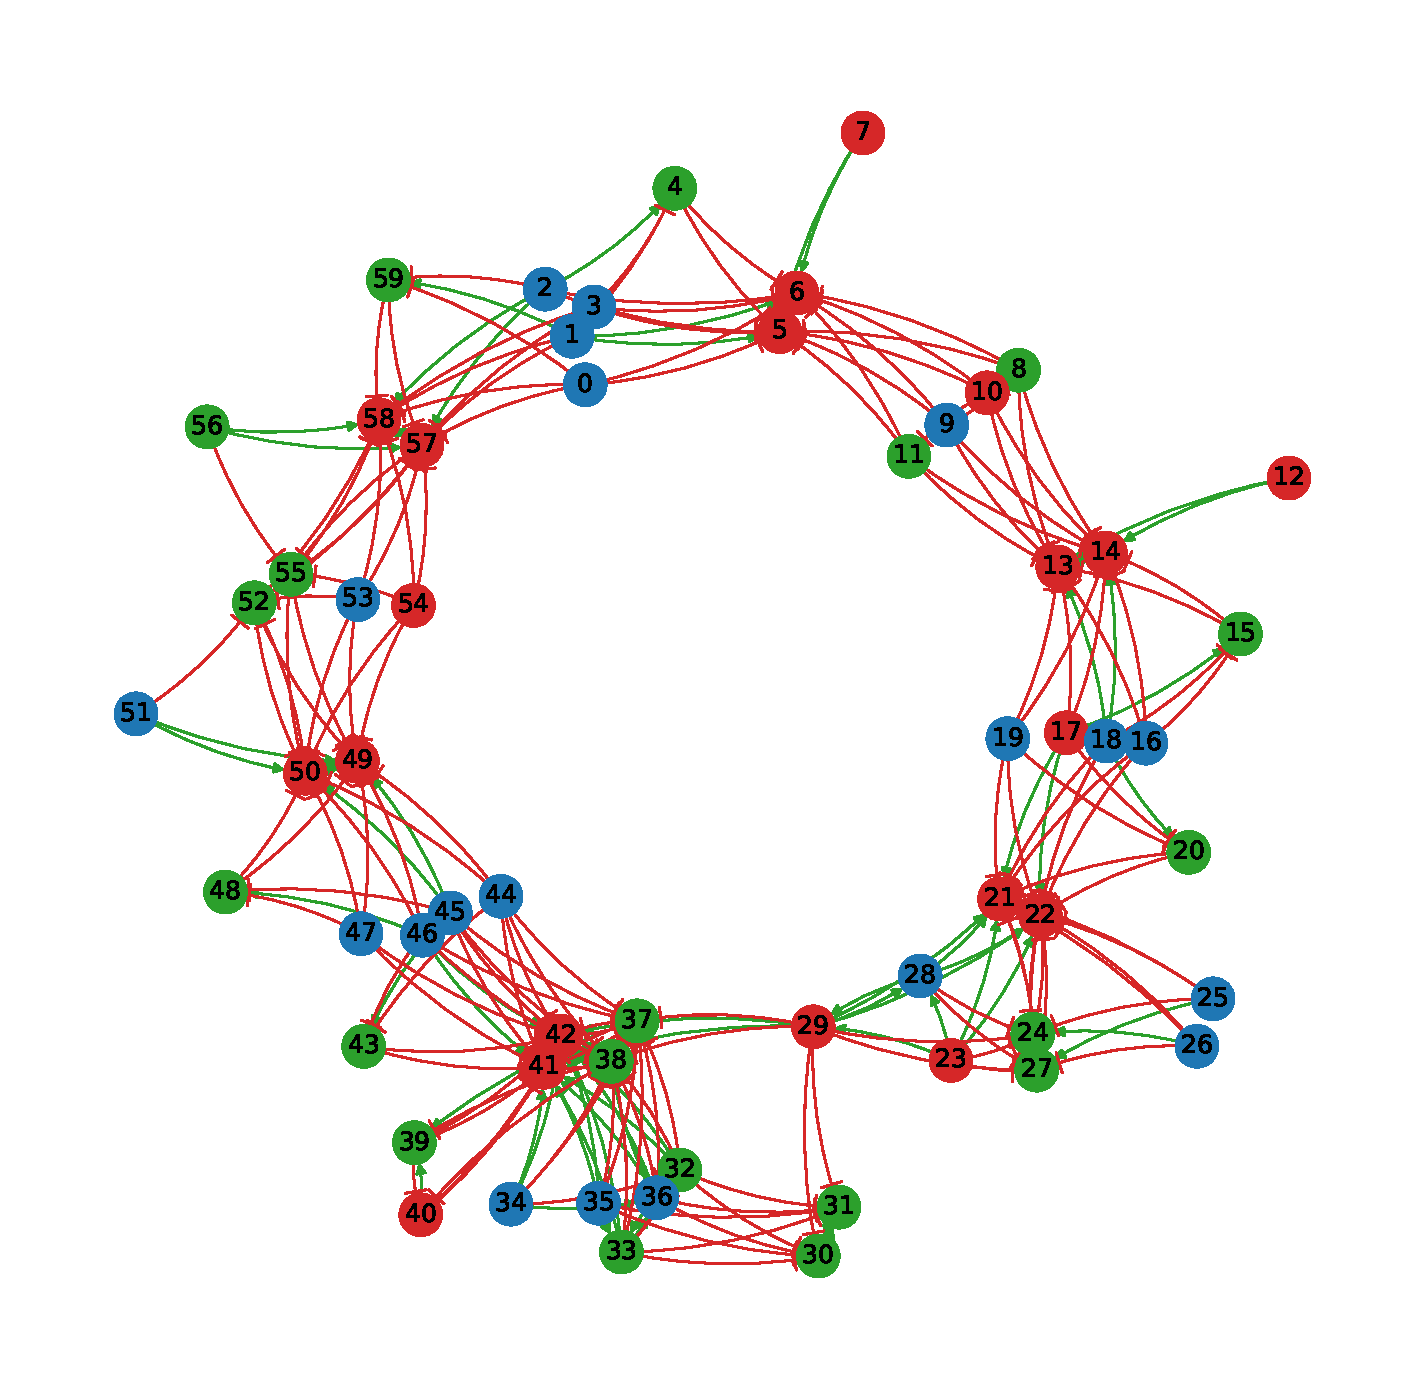
\includegraphics[width=0.75\textwidth]{ploscb/img/combined_effective_graph_rep21_graphviz.pdf}
  \caption{Effective interaction graph of the best individual at the end of replicate 21, obtained by knocking out each gene and measuring the resulting switches in activation levels in each environment.
  Activation edges are drawn in green, and inhibition edges in red.
  The numbering of the genes is the same as in Figures~\ref{fig:genomes} and~\ref{fig:ko_genomes}.}
  \label{fig:ko_graph}
\end{figure}

\paragraph{Building Effective Interaction Graphs}
In order to compute the effective interaction graph, we simply add an edge from a gene to every other gene whose activation state is switched by knocking out the first gene, in either environment.
If the knock-out inhibits a previously activated gene, we mark the edge as an activation edge, and we mark the edge as an inhibition edge if the knock-out activates a previously inhibited gene.
If knocking out a gene switches the same gene in the two environments, we only add the edge once (in other terms, we do not build a multigraph).
The result of constructing this graph, for the same individual, is presented in Figure~\ref{fig:ko_graph}.
In the case of this individual, there is a single weakly connected component, meaning that all genes interact in a genome-wide gene regulatory network.

\paragraph{Structure of Effective Interaction Graphs}
We computed the effective interaction graph of the best individual in each replicate, and compared these graphs with the effective interaction graphs of 30 random individuals drawn using the same genome parameters.
The results are presented in Figure~\ref{fig:ko_data}.
The effective interaction graphs of evolved individuals are clearly different from the interaction graphs of random individuals.
On the left-hand side of the figure, we can see that 26 out of the 30 evolved replicates have only one weakly connected component (WCC), which comprises every gene on the genome, while the remaining four have only one or two genes isolated from the main WCC.
On the other hand, WCC sizes in the random genomes span the whole range from single-gene to whole-genome weakly connected components.

\begin{figure}[H]
  \begin{subfigure}[t]{0.49\textwidth}
    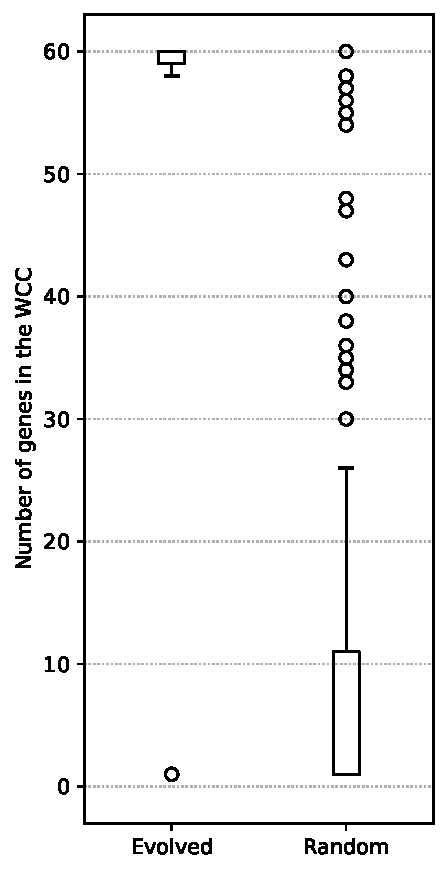
\includegraphics[width=\textwidth]{ploscb/img/effective_graph_wcc_distr.pdf}
  \end{subfigure}
  \begin{subfigure}[t]{0.49\textwidth}
    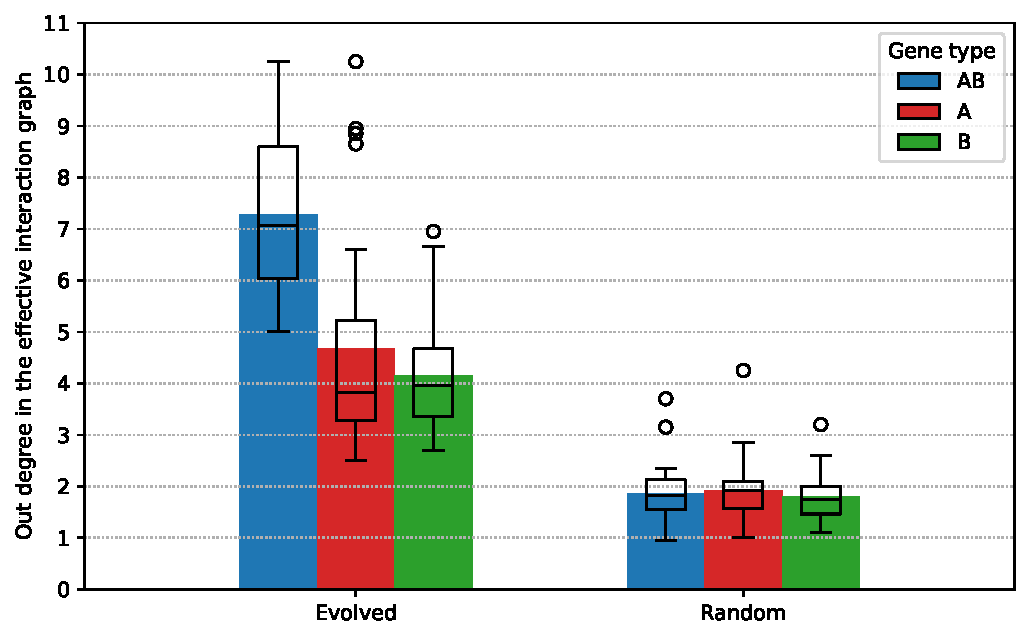
\includegraphics[width=\textwidth]{ploscb/img/effective_graph_combined_out_degree.pdf}
  \end{subfigure}
  \caption{Left: distribution of weakly connected component (WCC) sizes in the effective interaction graphs of the evolved individuals (left) and the random individuals (right).
  Right: average out-degree (number of genes switched by knocking-out a gene) of the nodes in the effective interaction graph, separated by gene type, for evolved and random individuals.}
  \label{fig:ko_data}
\end{figure}

The evolved genomes are indeed much more connected than the random genomes, as is shown on the right-hand side of Figure~\ref{fig:ko_data}.
While knocking out a gene in a random genome switches the state of just under two other genes on average, the figure is much higher in the evolved genomes.
Knocking out \emph{A} and \emph{B} genes switches on average four other genes, and knocking out \emph{AB} up to seven other genes; the higher out-degree of \emph{AB} genes in the graph was expected, as they are activated in both environments, while most \emph{A} and \emph{B} are inhibited in one environment or the other.

The effective gene regulatory network that emerges from the transcription-supercoiling coupling in our model therefore groups the whole genome into a single component that encompasses the whole genome, rather than a juxtaposition of independent subnetworks.

\section{Discussion and Perspectives}

% Note: talk about Visser 2022 in the intro?

DNA supercoiling is an important regulator of gene transcription in bacteria, mainly through its effect on promoter activation~\citep{forquet2021}, and plays a role in the rapid response of bacteria to changing environmental conditions~\citep{martisb.2019}.
The twin-domain model of transcription presented in~\cite{liu1987} and experimentally validated (most recently) in~\cite{visser2022} creates a bridge in the other direction, describing how gene transcription affects DNA supercoiling, giving rise to the transcription-supercoiling coupling.

In this work, we presented an evolutionary model of the transcription-supercoiling coupling (expanding upon our earlier work in~\cite{grohens2021}), in which populations of individuals must evolve differentiated gene expression levels via the coupling in response to different environmental conditions.
We developed this model in order to assess the theoretical possibility of the evolution of a gene regulatory network solely based on the coupling of the transcription levels of neighboring genes through DNA supercoiling, and to determine the potential evolutionary consequences of the evolution of such a regulatory network on genome structure.

We showed that, in this model, gene regulation by DNA supercoiling is indeed enough to evolve environment- and gene-class-specific patterns of gene transcription.
In particular, we observed the emergence of relaxation-activated genes, even though DNA relaxation always decreases promoter activity in the model; this provides a possible causal mechanism for the activity of genes found in \emph{E. coli} that display the same behavior~\citep{peter2004}.
We found that evolved genomes in the model are enriched in divergent pairs of always-active genes, echoing experimental data from \emph{E. coli}~\citep{sobetzko2016}; furthermore, convergent pairs can act as bistable toggle switches, mirroring theoretical predictions from models that explicitly describe the movement of RNA polymerases during gene transcription~\citep{sevier2021}.
Then, we showed that the local organization of the genome into convergent, divergent or tandem pairs is not enough to explain the transcriptional response to different environments, but that larger subnetworks can be required to inhibit genes.
Such regulation of gene expression through interaction with groups of neighboring genes could help explain the evolutionary persistence of synteny groups between \emph{E. coli} and \emph{S. enterica}~\citep{junier2016}, as genomic rearrangements would perturb the gene regulatory network created by these syntenies.
Finally, we characterized the gene regulatory networks in detail using gene knockouts, and showed that they span the whole genome of evolved individuals, in opposition to the sparser, disconnected regulatory networks displayed by randomly generated individuals.

Several further work directions remain open to investigation.
The experimental framework in which we tested our model remains very simple, and could be extended.
The desired gene expression levels in our model are binary, targeting maximal or minimal transcription, but could be replaced by any arbitrary level between these values for each gene, in order to see whether the local organization into pairs as well as the genome-wide gene regulatory network that we described are preserved under these less constrained conditions.
Similarly, we could refine the environmental challenge faced by individuals by evaluating them in each environment in succession, rather than separately, or by continuously changing the environment over evolutionary time.
From a theoretical perspective, a range of mechanistic biophysical models of the transcription-supercoiling coupling have been put forward, with varying levels of abstraction:~\cite{brackley2016} shows a phase transition in the transcription regime as the number of polymerases increases;~\cite{sevier2021} shows that bursty transcription can emerge from the transcription-supercoiling coupling; and ~\cite{meyer2014} and ~\cite{elhoudaigui2019} try to predict gene expression levels quantitatively from the local DNA supercoiling level.
It would therefore be an important vindication of the theoretical approach to the interplay between supercoiling and transcription to verify the extent to which these models, including ours, conform to one another as the level of abstraction changes.
Furthermore, integrating a model of gene regulation by DNA supercoiling into a more comprehensive evolutionary model of the genome that allows for classical gene regulation via transcription factors, such as Raevol~\citep{vadee-le-brun2016}, would shed light on the coevolution between different modes of gene regulation, and could help explain the link between genome size and regulation network complexity, especially in bacteria with reduced genomes such as \emph{B. aphidicola}~\citep{brinza2013}.
Finally, a better understanding of the regulatory interactions caused by the transcription-supercoiling coupling could help design more reliable synthetic genetic constructs, as explored in~\cite{johnstone2022}.
